\documentclass[8pt]{beamer}

\usepackage[french]{babel}
\usepackage[utf8]{inputenc}
\usepackage[T1]{fontenc}
\usepackage{amsmath}
\usepackage{mathdots}
\usepackage{yhmath}
\usepackage{cancel}
\usepackage{siunitx}
\usepackage{array}
\usepackage{multirow}
\usepackage{amssymb}
\usepackage{gensymb}
\usepackage{tabularx}
\usepackage{booktabs}
\usepackage{amsthm}
\usepackage{mathrsfs}
\usepackage{amsfonts}
\usepackage{stmaryrd}
\usepackage{xfrac}
\usepackage{dsfont}
\usepackage{fancybox}
\usepackage{multicol}
\usepackage{color}


\usepackage{lmodern}
\usepackage{tikz}
\usetikzlibrary{fadings}
\usetikzlibrary{patterns}
\usetikzlibrary{shadows.blur}
\usepackage{wrapfig}

\newcommand{\tabitem}{%
  \usebeamertemplate{itemize item}\hspace*{\labelsep}}

\usetheme{Warsaw}

\title[IA et conduite autonome]{Utilisation de l'intelligence artificielle dans la manœuvre autonome de bateau}
\author{Maxime CAUTRÈS}
\institute{Lycée Blaise Pascal}
\date{01/03/2020}


\AtBeginSection[]
{
  \begin{frame}
  \frametitle{Sommaire}
  \tableofcontents[currentsection, hideothersubsections]
  \end{frame} 
}

%\logo{
\includegraphics[height=10mm]{logo_limos_coul_def.png}}
%\logo{
\includegraphics[height=15mm]{logo_noir.png}}
\logo{
\includegraphics[height=10mm]{Logo-UCA.png}}


\begin{document}

\begin{frame}
  \titlepage
\end{frame}


\section{Introduction}

\subsection{Mise en contexte}


\begin{frame}{allowframebreaks}{\label{deb}}
  
  \frametitle{Données économiques}
  \begin{figure}
    \begin{center}
      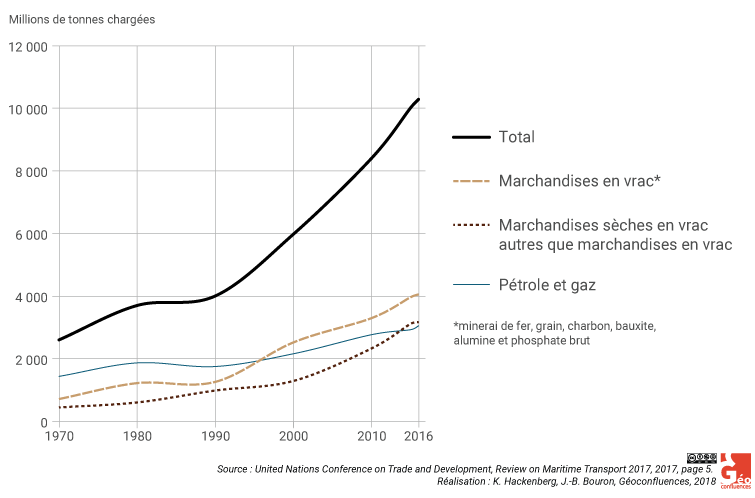
\includegraphics[height=50mm]{courbe_evo_bateau.png}
      \caption{La croissance du commerce maritime international (en millions de tonnes chargées) \footnote{http://geoconfluences.ens-lyon.fr/informations-scientifiques/dossiers-regionaux/territoires-europeens-regions-etats-union/rte-t/port-anvers}}
    \end{center}
  \end{figure}
  
\end{frame}


\begin{frame}
  \frametitle{Le métier de pilote maritime}

  \begin{figure}
    \begin{minipage}[c]{.52\linewidth}
        \centering
        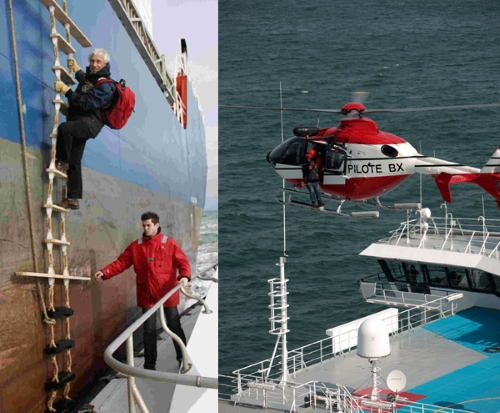
\includegraphics[height=5cm]{pilotemaritime.jpg}
        \caption{Transfert du pilote maritime sur le bateau à piloter \footnotemark}
    \end{minipage}
    \hfill%
    \begin{minipage}[c]{.40\linewidth}
        \centering
        \begin{itemize}
        \item Un métier \textbf{dangereux} (Le transfère du pilote)\break
          \pause
        \item Un \textbf{coût matériel} important (Bateau ou hélicoptère)\break
          \pause
        \item Un \textbf{coût financier} important (7\% du coût de l'escale)
        \end{itemize}
    \end{minipage}
    \footnotetext{http://escale.sinerj.org/spip.php?article41}
\end{figure}
  
\end{frame}


\begin{frame}
  \frametitle{Étude de l'existant}

   \begin{figure}
    \begin{minipage}[c]{.46\linewidth}
        \centering
        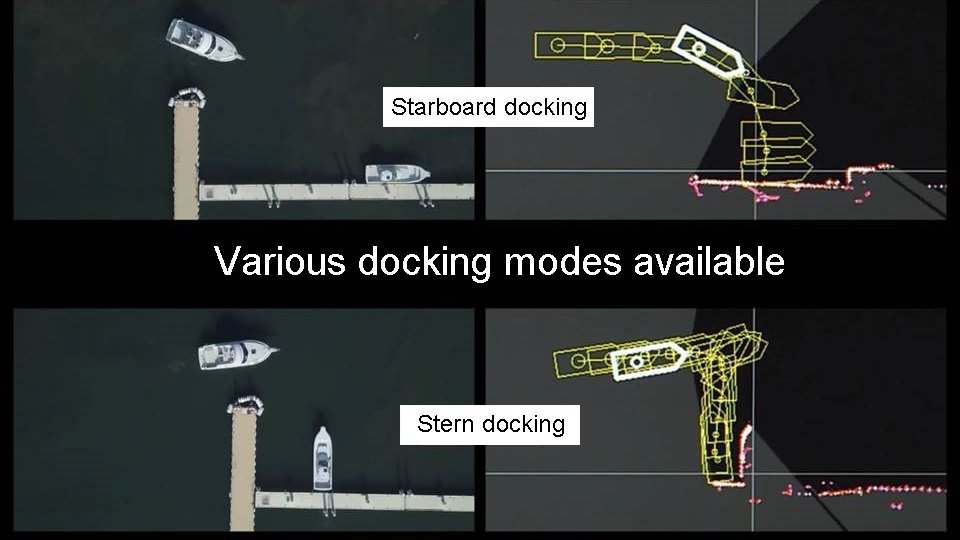
\includegraphics[width=55mm]{boat_docking.jpg}
        \caption{Vu aérienne de la trajectoire suivit par l'asservissement du bateau \footnotemark}
    \end{minipage}
    \footnotetext{https://smartmaritimenetwork.com/2019/02/08/yanmar-trials-robotic-ship-technology/}
    \hfill%
    \begin{minipage}[c]{.46\linewidth}
        \centering
        \begin{itemize}
        \item \textbf{Peu d'acteurs} dans le domaine (Deux principaux avec Yanmar et Volvo) \break
          \pause
        \item Nécessite des modifications importantes des \textbf{infrastructures} (capteurs, antennes) \break
          \pause
        \item Un dispositif \textbf{très lent et peu adapté} aux déplacements important dans un port 
        \end{itemize}
    \end{minipage}
     
\end{figure}
\end{frame}

\subsection{Une nouvelle approche}

\begin{frame}

  \frametitle{L'apprentissage automatique:}

  \begin{figure}
    \begin{minipage}[c]{.46\linewidth}
      \centering
      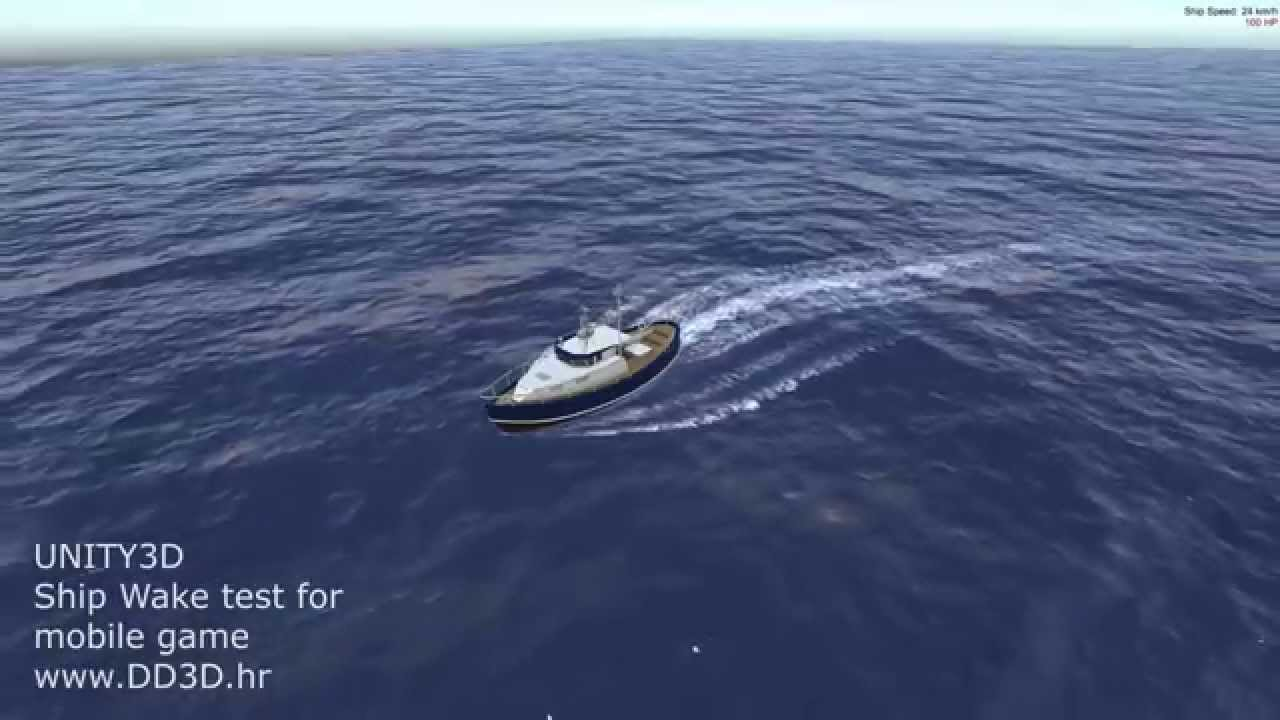
\includegraphics[width=55mm]{simulation_boat.jpg}
    \end{minipage}
    \hfill%
    \begin{minipage}[c]{.46\linewidth}
      \centering
      \begin{itemize}
  \item Un environnement pour simuler les conditions réelles \break
    \break \break \break
  \end{itemize}
    \end{minipage}
  \end{figure}

\end{frame}
  
\begin{frame}

  \frametitle{L'apprentissage automatique:}

  \begin{figure}
    \begin{minipage}[c]{.46\linewidth}
      \centering
      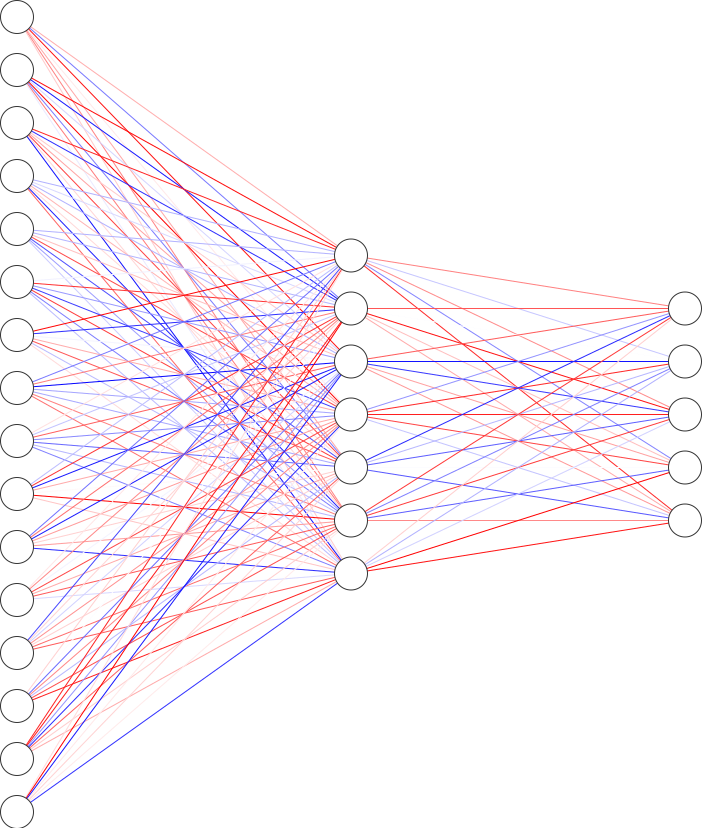
\includegraphics[width=45mm]{network_example.png}
    \end{minipage}
    \hfill%
    \begin{minipage}[c]{.46\linewidth}
      \centering
      \begin{itemize}
  \item Un environnement  \break
  \item La techonologie des réseaux de neuronnes\break
    \pause
  \item Des algorithmes d'entrainement
  \end{itemize}
    \end{minipage}
  \end{figure}

\end{frame}

\subsection{Problématique}

\begin{frame}

  \frametitle{Problématique}
  
  Comment peut-on utiliser l’\textbf{apprentissage automatique} pour
  permettre à un bateau de \textbf{manœuvrer dans un port} dans le but de
  minimiser les dépenses liées à l’augmentation du trafic tout en
  garantissant la sécurité ?
  \break \pause
  \begin{center}
    \begin{tabular}{@{}l@{}}
      Le plan: \\ \\ 
      \pause
      \tabitem Première approche avec le Q-learning \\ \\
      \pause
      \tabitem Simulation de l'environnement portuaire \\ \\
      \pause
      \tabitem Seconde approche avec le Policy Gradients
    \end{tabular}
    \end{center}
\end{frame}



\section{Le Q-learning}
\subsection{Le problème des souris}

\begin{frame}{allowframebreaks}{\label{2}}
  \frametitle{Un problème intermédiaire pour se lancer}
  \framesubtitle{Description}

  \begin{figure}
    \begin{minipage}[c]{.46\linewidth}
      \centering
      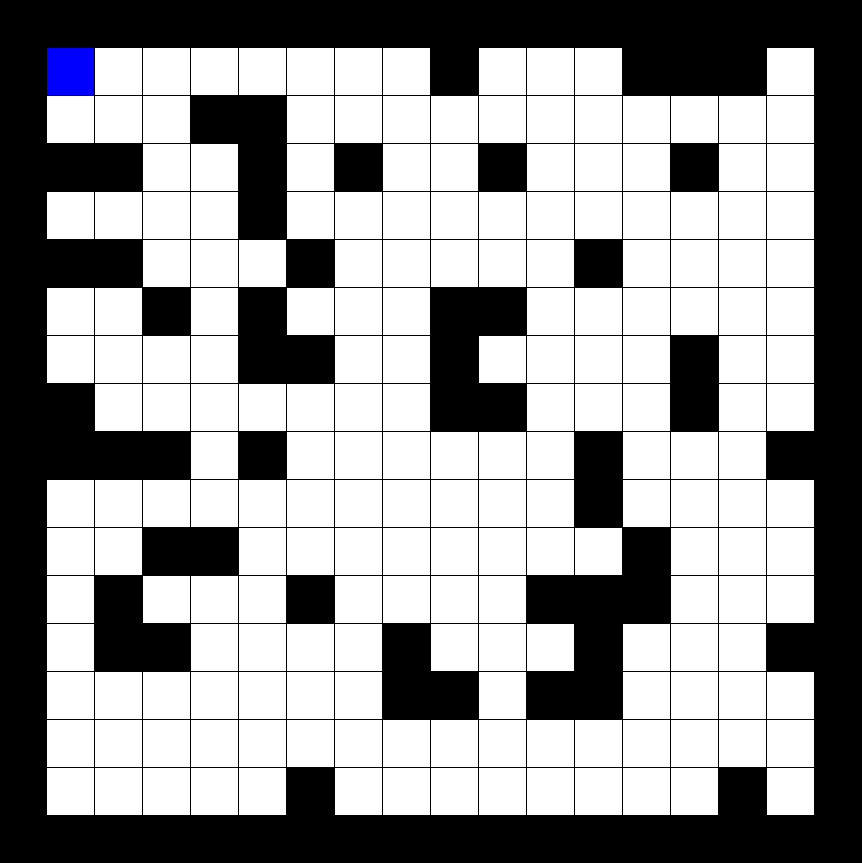
\includegraphics[width=45mm]{map_q-learning.png}
    \end{minipage}
    \hfill%
    \begin{minipage}[c]{.46\linewidth}
      \centering
      \begin{itemize}
      \item En Noir les obstacles \break
      \item En blanc les cases accessibles \break
      \item La souris est en bleu \break
      \item L'objectif en la case en bas a droite \break
  \end{itemize}
    \end{minipage}
  \end{figure}
 
\end{frame}

\begin{frame}{allowframebreaks}{\label{2}}
  \frametitle{Un problème intermédiaire pour se lancer}
  \framesubtitle{Formalisation}
  \begin{figure}
    \begin{minipage}[c]{.55\linewidth}
      \centering
      
\tikzset{every picture/.style={line width=0.75pt}} %set default line width to 0.75pt        

\begin{tikzpicture}[x=0.75pt,y=0.75pt,yscale=-1,xscale=1]
%uncomment if require: \path (0,461); %set diagram left start at 0, and has height of 461

%Shape: Circle [id:dp8540746348453063] 
\draw  [fill={rgb, 255:red, 74; green, 144; blue, 226 }  ,fill opacity=1 ] (102.51,57.17) .. controls (102.32,47.69) and (109.85,40) .. (119.33,40) .. controls (128.81,40) and (136.65,47.69) .. (136.84,57.17) .. controls (137.03,66.65) and (129.5,74.33) .. (120.02,74.33) .. controls (110.54,74.33) and (102.7,66.65) .. (102.51,57.17) -- cycle ;
%Shape: Circle [id:dp06819830701291374] 
\draw   (162.51,57.17) .. controls (162.32,47.69) and (169.85,40) .. (179.33,40) .. controls (188.81,40) and (196.65,47.69) .. (196.84,57.17) .. controls (197.03,66.65) and (189.5,74.33) .. (180.02,74.33) .. controls (170.54,74.33) and (162.7,66.65) .. (162.51,57.17) -- cycle ;
%Shape: Circle [id:dp6404605832115242] 
\draw   (222.51,57.17) .. controls (222.32,47.69) and (229.85,40) .. (239.33,40) .. controls (248.81,40) and (256.65,47.69) .. (256.84,57.17) .. controls (257.03,66.65) and (249.5,74.33) .. (240.02,74.33) .. controls (230.54,74.33) and (222.7,66.65) .. (222.51,57.17) -- cycle ;
%Shape: Circle [id:dp8151459352121608] 
\draw  [fill={rgb, 255:red, 208; green, 2; blue, 27 }  ,fill opacity=1 ] (282.51,57.17) .. controls (282.32,47.69) and (289.85,40) .. (299.33,40) .. controls (308.81,40) and (316.65,47.69) .. (316.84,57.17) .. controls (317.03,66.65) and (309.5,74.33) .. (300.02,74.33) .. controls (290.54,74.33) and (282.7,66.65) .. (282.51,57.17) -- cycle ;
%Shape: Circle [id:dp3137705827724606] 
\draw   (102.51,116.17) .. controls (102.32,106.69) and (109.85,99) .. (119.33,99) .. controls (128.81,99) and (136.65,106.69) .. (136.84,116.17) .. controls (137.03,125.65) and (129.5,133.33) .. (120.02,133.33) .. controls (110.54,133.33) and (102.7,125.65) .. (102.51,116.17) -- cycle ;
%Shape: Circle [id:dp42706265444246716] 
\draw   (162.51,116.17) .. controls (162.32,106.69) and (169.85,99) .. (179.33,99) .. controls (188.81,99) and (196.65,106.69) .. (196.84,116.17) .. controls (197.03,125.65) and (189.5,133.33) .. (180.02,133.33) .. controls (170.54,133.33) and (162.7,125.65) .. (162.51,116.17) -- cycle ;
%Shape: Circle [id:dp04194321843609039] 
\draw  [fill={rgb, 255:red, 208; green, 2; blue, 27 }  ,fill opacity=1 ] (222.51,116.17) .. controls (222.32,106.69) and (229.85,99) .. (239.33,99) .. controls (248.81,99) and (256.65,106.69) .. (256.84,116.17) .. controls (257.03,125.65) and (249.5,133.33) .. (240.02,133.33) .. controls (230.54,133.33) and (222.7,125.65) .. (222.51,116.17) -- cycle ;
%Shape: Circle [id:dp5402564916898607] 
\draw  [fill={rgb, 255:red, 208; green, 2; blue, 27 }  ,fill opacity=1 ] (282.51,116.17) .. controls (282.32,106.69) and (289.85,99) .. (299.33,99) .. controls (308.81,99) and (316.65,106.69) .. (316.84,116.17) .. controls (317.03,125.65) and (309.5,133.33) .. (300.02,133.33) .. controls (290.54,133.33) and (282.7,125.65) .. (282.51,116.17) -- cycle ;
%Shape: Circle [id:dp12224593593474364] 
\draw  [fill={rgb, 255:red, 208; green, 2; blue, 27 }  ,fill opacity=1 ] (102.51,175.17) .. controls (102.32,165.69) and (109.85,158) .. (119.33,158) .. controls (128.81,158) and (136.65,165.69) .. (136.84,175.17) .. controls (137.03,184.65) and (129.5,192.33) .. (120.02,192.33) .. controls (110.54,192.33) and (102.7,184.65) .. (102.51,175.17) -- cycle ;
%Shape: Circle [id:dp7140336825967974] 
\draw  [fill={rgb, 255:red, 239; green, 20; blue, 20 }  ,fill opacity=0 ] (162.51,175.17) .. controls (162.32,165.69) and (169.85,158) .. (179.33,158) .. controls (188.81,158) and (196.65,165.69) .. (196.84,175.17) .. controls (197.03,184.65) and (189.5,192.33) .. (180.02,192.33) .. controls (170.54,192.33) and (162.7,184.65) .. (162.51,175.17) -- cycle ;
%Shape: Circle [id:dp30642985177667037] 
\draw   (222.51,175.17) .. controls (222.32,165.69) and (229.85,158) .. (239.33,158) .. controls (248.81,158) and (256.65,165.69) .. (256.84,175.17) .. controls (257.03,184.65) and (249.5,192.33) .. (240.02,192.33) .. controls (230.54,192.33) and (222.7,184.65) .. (222.51,175.17) -- cycle ;
%Shape: Circle [id:dp327707847282138] 
\draw   (282.51,175.17) .. controls (282.32,165.69) and (289.85,158) .. (299.33,158) .. controls (308.81,158) and (316.65,165.69) .. (316.84,175.17) .. controls (317.03,184.65) and (309.5,192.33) .. (300.02,192.33) .. controls (290.54,192.33) and (282.7,184.65) .. (282.51,175.17) -- cycle ;
%Shape: Circle [id:dp8649323540938678] 
\draw  [fill={rgb, 255:red, 208; green, 2; blue, 27 }  ,fill opacity=1 ] (102.51,234.17) .. controls (102.32,224.69) and (109.85,217) .. (119.33,217) .. controls (128.81,217) and (136.65,224.69) .. (136.84,234.17) .. controls (137.03,243.65) and (129.5,251.33) .. (120.02,251.33) .. controls (110.54,251.33) and (102.7,243.65) .. (102.51,234.17) -- cycle ;
%Shape: Circle [id:dp9368241553908816] 
\draw   (162.51,234.17) .. controls (162.32,224.69) and (169.85,217) .. (179.33,217) .. controls (188.81,217) and (196.65,224.69) .. (196.84,234.17) .. controls (197.03,243.65) and (189.5,251.33) .. (180.02,251.33) .. controls (170.54,251.33) and (162.7,243.65) .. (162.51,234.17) -- cycle ;
%Shape: Circle [id:dp7801501699877016] 
\draw  [fill={rgb, 255:red, 208; green, 2; blue, 27 }  ,fill opacity=1 ] (222.51,234.17) .. controls (222.32,224.69) and (229.85,217) .. (239.33,217) .. controls (248.81,217) and (256.65,224.69) .. (256.84,234.17) .. controls (257.03,243.65) and (249.5,251.33) .. (240.02,251.33) .. controls (230.54,251.33) and (222.7,243.65) .. (222.51,234.17) -- cycle ;
%Shape: Circle [id:dp7565141812931631] 
\draw  [fill={rgb, 255:red, 126; green, 211; blue, 33 }  ,fill opacity=1 ] (282.51,234.17) .. controls (282.32,224.69) and (289.85,217) .. (299.33,217) .. controls (308.81,217) and (316.65,224.69) .. (316.84,234.17) .. controls (317.03,243.65) and (309.5,251.33) .. (300.02,251.33) .. controls (290.54,251.33) and (282.7,243.65) .. (282.51,234.17) -- cycle ;
%Curve Lines [id:da730045195238507] 
\draw    (112.5,100) .. controls (108.72,86.77) and (109.41,84.26) .. (112.87,74.74) ;
\draw [shift={(113.5,73)}, rotate = 469.98] [color={rgb, 255:red, 0; green, 0; blue, 0 }  ][line width=0.75]    (10.93,-3.29) .. controls (6.95,-1.4) and (3.31,-0.3) .. (0,0) .. controls (3.31,0.3) and (6.95,1.4) .. (10.93,3.29)   ;
%Curve Lines [id:da09407301633088849] 
\draw    (172.5,100) .. controls (168.72,86.77) and (169.41,84.26) .. (172.87,74.74) ;
\draw [shift={(173.5,73)}, rotate = 469.98] [color={rgb, 255:red, 0; green, 0; blue, 0 }  ][line width=0.75]    (10.93,-3.29) .. controls (6.95,-1.4) and (3.31,-0.3) .. (0,0) .. controls (3.31,0.3) and (6.95,1.4) .. (10.93,3.29)   ;
%Curve Lines [id:da15643436871844396] 
\draw    (233.5,100) .. controls (229.72,86.77) and (230.41,84.26) .. (233.87,74.74) ;
\draw [shift={(234.5,73)}, rotate = 469.98] [color={rgb, 255:red, 0; green, 0; blue, 0 }  ][line width=0.75]    (10.93,-3.29) .. controls (6.95,-1.4) and (3.31,-0.3) .. (0,0) .. controls (3.31,0.3) and (6.95,1.4) .. (10.93,3.29)   ;
%Curve Lines [id:da0905869695635051] 
\draw    (293.5,100) .. controls (289.72,86.77) and (290.41,84.26) .. (293.87,74.74) ;
\draw [shift={(294.5,73)}, rotate = 469.98] [color={rgb, 255:red, 0; green, 0; blue, 0 }  ][line width=0.75]    (10.93,-3.29) .. controls (6.95,-1.4) and (3.31,-0.3) .. (0,0) .. controls (3.31,0.3) and (6.95,1.4) .. (10.93,3.29)   ;
%Curve Lines [id:da3353755717935154] 
\draw    (307.91,72.7) .. controls (311.73,85.92) and (311.06,88.44) .. (307.62,97.97) ;
\draw [shift={(307,99.71)}, rotate = 289.79] [color={rgb, 255:red, 0; green, 0; blue, 0 }  ][line width=0.75]    (10.93,-3.29) .. controls (6.95,-1.4) and (3.31,-0.3) .. (0,0) .. controls (3.31,0.3) and (6.95,1.4) .. (10.93,3.29)   ;
%Curve Lines [id:da38934399199571446] 
\draw    (247.91,72.9) .. controls (250.05,80.3) and (250.78,84.34) .. (250.41,88.14) .. controls (250.12,91.1) and (249.15,93.92) .. (247.67,98.05) ;
\draw [shift={(247,99.9)}, rotate = 289.79] [color={rgb, 255:red, 0; green, 0; blue, 0 }  ][line width=0.75]    (10.93,-3.29) .. controls (6.95,-1.4) and (3.31,-0.3) .. (0,0) .. controls (3.31,0.3) and (6.95,1.4) .. (10.93,3.29)   ;
%Curve Lines [id:da34027139908583437] 
\draw    (186.91,73.1) .. controls (190.73,86.32) and (190.06,88.84) .. (186.63,98.37) ;
\draw [shift={(186,100.11)}, rotate = 289.79] [color={rgb, 255:red, 0; green, 0; blue, 0 }  ][line width=0.75]    (10.93,-3.29) .. controls (6.95,-1.4) and (3.31,-0.3) .. (0,0) .. controls (3.31,0.3) and (6.95,1.4) .. (10.93,3.29)   ;
%Curve Lines [id:da796991344875204] 
\draw    (126.91,73.3) .. controls (130.73,86.52) and (130.06,89.04) .. (126.63,98.57) ;
\draw [shift={(126,100.31)}, rotate = 289.79] [color={rgb, 255:red, 0; green, 0; blue, 0 }  ][line width=0.75]    (10.93,-3.29) .. controls (6.95,-1.4) and (3.31,-0.3) .. (0,0) .. controls (3.31,0.3) and (6.95,1.4) .. (10.93,3.29)   ;
%Curve Lines [id:da7201323904025818] 
\draw    (112.5,159) .. controls (108.72,145.77) and (109.41,143.26) .. (112.87,133.74) ;
\draw [shift={(113.5,132)}, rotate = 469.98] [color={rgb, 255:red, 0; green, 0; blue, 0 }  ][line width=0.75]    (10.93,-3.29) .. controls (6.95,-1.4) and (3.31,-0.3) .. (0,0) .. controls (3.31,0.3) and (6.95,1.4) .. (10.93,3.29)   ;
%Curve Lines [id:da20546300505258275] 
\draw    (172.5,159) .. controls (168.72,145.77) and (169.41,143.26) .. (172.87,133.74) ;
\draw [shift={(173.5,132)}, rotate = 469.98] [color={rgb, 255:red, 0; green, 0; blue, 0 }  ][line width=0.75]    (10.93,-3.29) .. controls (6.95,-1.4) and (3.31,-0.3) .. (0,0) .. controls (3.31,0.3) and (6.95,1.4) .. (10.93,3.29)   ;
%Curve Lines [id:da07581444069265886] 
\draw    (233.5,159) .. controls (229.72,145.77) and (230.41,143.26) .. (233.87,133.74) ;
\draw [shift={(234.5,132)}, rotate = 469.98] [color={rgb, 255:red, 0; green, 0; blue, 0 }  ][line width=0.75]    (10.93,-3.29) .. controls (6.95,-1.4) and (3.31,-0.3) .. (0,0) .. controls (3.31,0.3) and (6.95,1.4) .. (10.93,3.29)   ;
%Curve Lines [id:da29939537277929507] 
\draw    (293.5,159) .. controls (289.72,145.77) and (290.41,143.26) .. (293.87,133.74) ;
\draw [shift={(294.5,132)}, rotate = 469.98] [color={rgb, 255:red, 0; green, 0; blue, 0 }  ][line width=0.75]    (10.93,-3.29) .. controls (6.95,-1.4) and (3.31,-0.3) .. (0,0) .. controls (3.31,0.3) and (6.95,1.4) .. (10.93,3.29)   ;
%Curve Lines [id:da9084064621725036] 
\draw    (307.91,131.7) .. controls (311.73,144.92) and (311.06,147.44) .. (307.62,156.97) ;
\draw [shift={(307,158.71)}, rotate = 289.79] [color={rgb, 255:red, 0; green, 0; blue, 0 }  ][line width=0.75]    (10.93,-3.29) .. controls (6.95,-1.4) and (3.31,-0.3) .. (0,0) .. controls (3.31,0.3) and (6.95,1.4) .. (10.93,3.29)   ;
%Curve Lines [id:da6963722810275621] 
\draw    (247.91,131.9) .. controls (250.05,139.3) and (250.78,143.34) .. (250.41,147.14) .. controls (250.12,150.1) and (249.15,152.92) .. (247.67,157.05) ;
\draw [shift={(247,158.9)}, rotate = 289.79] [color={rgb, 255:red, 0; green, 0; blue, 0 }  ][line width=0.75]    (10.93,-3.29) .. controls (6.95,-1.4) and (3.31,-0.3) .. (0,0) .. controls (3.31,0.3) and (6.95,1.4) .. (10.93,3.29)   ;
%Curve Lines [id:da12750225999473463] 
\draw    (186.91,132.1) .. controls (190.73,145.32) and (190.06,147.84) .. (186.63,157.37) ;
\draw [shift={(186,159.11)}, rotate = 289.79] [color={rgb, 255:red, 0; green, 0; blue, 0 }  ][line width=0.75]    (10.93,-3.29) .. controls (6.95,-1.4) and (3.31,-0.3) .. (0,0) .. controls (3.31,0.3) and (6.95,1.4) .. (10.93,3.29)   ;
%Curve Lines [id:da27650032387185797] 
\draw    (126.91,132.3) .. controls (130.73,145.52) and (130.06,148.04) .. (126.63,157.57) ;
\draw [shift={(126,159.31)}, rotate = 289.79] [color={rgb, 255:red, 0; green, 0; blue, 0 }  ][line width=0.75]    (10.93,-3.29) .. controls (6.95,-1.4) and (3.31,-0.3) .. (0,0) .. controls (3.31,0.3) and (6.95,1.4) .. (10.93,3.29)   ;
%Curve Lines [id:da2459899481100294] 
\draw    (111.5,218) .. controls (107.72,204.77) and (108.41,202.26) .. (111.87,192.74) ;
\draw [shift={(112.5,191)}, rotate = 469.98] [color={rgb, 255:red, 0; green, 0; blue, 0 }  ][line width=0.75]    (10.93,-3.29) .. controls (6.95,-1.4) and (3.31,-0.3) .. (0,0) .. controls (3.31,0.3) and (6.95,1.4) .. (10.93,3.29)   ;
%Curve Lines [id:da46236537062468197] 
\draw    (171.5,218) .. controls (167.72,204.77) and (168.41,202.26) .. (171.87,192.74) ;
\draw [shift={(172.5,191)}, rotate = 469.98] [color={rgb, 255:red, 0; green, 0; blue, 0 }  ][line width=0.75]    (10.93,-3.29) .. controls (6.95,-1.4) and (3.31,-0.3) .. (0,0) .. controls (3.31,0.3) and (6.95,1.4) .. (10.93,3.29)   ;
%Curve Lines [id:da23098462238939543] 
\draw    (232.5,218) .. controls (228.72,204.77) and (229.41,202.26) .. (232.87,192.74) ;
\draw [shift={(233.5,191)}, rotate = 469.98] [color={rgb, 255:red, 0; green, 0; blue, 0 }  ][line width=0.75]    (10.93,-3.29) .. controls (6.95,-1.4) and (3.31,-0.3) .. (0,0) .. controls (3.31,0.3) and (6.95,1.4) .. (10.93,3.29)   ;
%Curve Lines [id:da14951842056084663] 
\draw    (292.5,218) .. controls (288.72,204.77) and (289.41,202.26) .. (292.87,192.74) ;
\draw [shift={(293.5,191)}, rotate = 469.98] [color={rgb, 255:red, 0; green, 0; blue, 0 }  ][line width=0.75]    (10.93,-3.29) .. controls (6.95,-1.4) and (3.31,-0.3) .. (0,0) .. controls (3.31,0.3) and (6.95,1.4) .. (10.93,3.29)   ;
%Curve Lines [id:da44770102947153356] 
\draw    (306.91,190.7) .. controls (310.73,203.92) and (310.06,206.44) .. (306.62,215.97) ;
\draw [shift={(306,217.71)}, rotate = 289.79] [color={rgb, 255:red, 0; green, 0; blue, 0 }  ][line width=0.75]    (10.93,-3.29) .. controls (6.95,-1.4) and (3.31,-0.3) .. (0,0) .. controls (3.31,0.3) and (6.95,1.4) .. (10.93,3.29)   ;
%Curve Lines [id:da33045625698784753] 
\draw    (246.91,190.9) .. controls (249.05,198.3) and (249.78,202.34) .. (249.41,206.14) .. controls (249.12,209.1) and (248.15,211.92) .. (246.67,216.05) ;
\draw [shift={(246,217.9)}, rotate = 289.79] [color={rgb, 255:red, 0; green, 0; blue, 0 }  ][line width=0.75]    (10.93,-3.29) .. controls (6.95,-1.4) and (3.31,-0.3) .. (0,0) .. controls (3.31,0.3) and (6.95,1.4) .. (10.93,3.29)   ;
%Curve Lines [id:da3574921477134665] 
\draw    (185.91,191.1) .. controls (189.73,204.32) and (189.06,206.84) .. (185.63,216.37) ;
\draw [shift={(185,218.11)}, rotate = 289.79] [color={rgb, 255:red, 0; green, 0; blue, 0 }  ][line width=0.75]    (10.93,-3.29) .. controls (6.95,-1.4) and (3.31,-0.3) .. (0,0) .. controls (3.31,0.3) and (6.95,1.4) .. (10.93,3.29)   ;
%Curve Lines [id:da8636386180501088] 
\draw    (125.91,191.3) .. controls (129.73,204.52) and (129.06,207.04) .. (125.63,216.57) ;
\draw [shift={(125,218.31)}, rotate = 289.79] [color={rgb, 255:red, 0; green, 0; blue, 0 }  ][line width=0.75]    (10.93,-3.29) .. controls (6.95,-1.4) and (3.31,-0.3) .. (0,0) .. controls (3.31,0.3) and (6.95,1.4) .. (10.93,3.29)   ;
%Curve Lines [id:da1526901261154867] 
\draw    (135.28,49.75) .. controls (148.44,45.74) and (150.97,46.39) .. (160.54,49.68) ;
\draw [shift={(162.29,50.28)}, rotate = 198.98] [color={rgb, 255:red, 0; green, 0; blue, 0 }  ][line width=0.75]    (10.93,-3.29) .. controls (6.95,-1.4) and (3.31,-0.3) .. (0,0) .. controls (3.31,0.3) and (6.95,1.4) .. (10.93,3.29)   ;
%Curve Lines [id:da11671625142080866] 
\draw    (163.22,64.7) .. controls (150.07,68.75) and (147.55,68.12) .. (137.96,64.85) ;
\draw [shift={(136.21,64.26)}, rotate = 378.78999999999996] [color={rgb, 255:red, 0; green, 0; blue, 0 }  ][line width=0.75]    (10.93,-3.29) .. controls (6.95,-1.4) and (3.31,-0.3) .. (0,0) .. controls (3.31,0.3) and (6.95,1.4) .. (10.93,3.29)   ;
%Curve Lines [id:da5484140250658931] 
\draw    (135.28,108.75) .. controls (148.44,104.74) and (150.97,105.39) .. (160.54,108.68) ;
\draw [shift={(162.29,109.28)}, rotate = 198.98] [color={rgb, 255:red, 0; green, 0; blue, 0 }  ][line width=0.75]    (10.93,-3.29) .. controls (6.95,-1.4) and (3.31,-0.3) .. (0,0) .. controls (3.31,0.3) and (6.95,1.4) .. (10.93,3.29)   ;
%Curve Lines [id:da7986949791784275] 
\draw    (163.22,123.7) .. controls (150.07,127.75) and (147.55,127.12) .. (137.96,123.85) ;
\draw [shift={(136.21,123.26)}, rotate = 378.78999999999996] [color={rgb, 255:red, 0; green, 0; blue, 0 }  ][line width=0.75]    (10.93,-3.29) .. controls (6.95,-1.4) and (3.31,-0.3) .. (0,0) .. controls (3.31,0.3) and (6.95,1.4) .. (10.93,3.29)   ;
%Curve Lines [id:da6788885031884317] 
\draw    (135.28,167.75) .. controls (148.44,163.74) and (150.97,164.39) .. (160.54,167.68) ;
\draw [shift={(162.29,168.28)}, rotate = 198.98] [color={rgb, 255:red, 0; green, 0; blue, 0 }  ][line width=0.75]    (10.93,-3.29) .. controls (6.95,-1.4) and (3.31,-0.3) .. (0,0) .. controls (3.31,0.3) and (6.95,1.4) .. (10.93,3.29)   ;
%Curve Lines [id:da09559530421739137] 
\draw    (163.22,182.7) .. controls (150.07,186.75) and (147.55,186.12) .. (137.96,182.85) ;
\draw [shift={(136.21,182.26)}, rotate = 378.78999999999996] [color={rgb, 255:red, 0; green, 0; blue, 0 }  ][line width=0.75]    (10.93,-3.29) .. controls (6.95,-1.4) and (3.31,-0.3) .. (0,0) .. controls (3.31,0.3) and (6.95,1.4) .. (10.93,3.29)   ;
%Curve Lines [id:da2985355825508491] 
\draw    (135.28,226.75) .. controls (148.44,222.74) and (150.97,223.39) .. (160.54,226.68) ;
\draw [shift={(162.29,227.28)}, rotate = 198.98] [color={rgb, 255:red, 0; green, 0; blue, 0 }  ][line width=0.75]    (10.93,-3.29) .. controls (6.95,-1.4) and (3.31,-0.3) .. (0,0) .. controls (3.31,0.3) and (6.95,1.4) .. (10.93,3.29)   ;
%Curve Lines [id:da40118124459654747] 
\draw    (163.22,241.7) .. controls (150.07,245.75) and (147.55,245.12) .. (137.96,241.85) ;
\draw [shift={(136.21,241.26)}, rotate = 378.78999999999996] [color={rgb, 255:red, 0; green, 0; blue, 0 }  ][line width=0.75]    (10.93,-3.29) .. controls (6.95,-1.4) and (3.31,-0.3) .. (0,0) .. controls (3.31,0.3) and (6.95,1.4) .. (10.93,3.29)   ;
%Curve Lines [id:da7967268933492142] 
\draw    (195.28,49.75) .. controls (208.44,45.74) and (210.97,46.39) .. (220.54,49.68) ;
\draw [shift={(222.29,50.28)}, rotate = 198.98] [color={rgb, 255:red, 0; green, 0; blue, 0 }  ][line width=0.75]    (10.93,-3.29) .. controls (6.95,-1.4) and (3.31,-0.3) .. (0,0) .. controls (3.31,0.3) and (6.95,1.4) .. (10.93,3.29)   ;
%Curve Lines [id:da6624834675485927] 
\draw    (223.22,64.7) .. controls (210.07,68.75) and (207.55,68.12) .. (197.96,64.85) ;
\draw [shift={(196.21,64.26)}, rotate = 378.78999999999996] [color={rgb, 255:red, 0; green, 0; blue, 0 }  ][line width=0.75]    (10.93,-3.29) .. controls (6.95,-1.4) and (3.31,-0.3) .. (0,0) .. controls (3.31,0.3) and (6.95,1.4) .. (10.93,3.29)   ;
%Curve Lines [id:da37269297103592036] 
\draw    (195.28,108.75) .. controls (208.44,104.74) and (210.97,105.39) .. (220.54,108.68) ;
\draw [shift={(222.29,109.28)}, rotate = 198.98] [color={rgb, 255:red, 0; green, 0; blue, 0 }  ][line width=0.75]    (10.93,-3.29) .. controls (6.95,-1.4) and (3.31,-0.3) .. (0,0) .. controls (3.31,0.3) and (6.95,1.4) .. (10.93,3.29)   ;
%Curve Lines [id:da8649419749215743] 
\draw    (223.22,123.7) .. controls (210.07,127.75) and (207.55,127.12) .. (197.96,123.85) ;
\draw [shift={(196.21,123.26)}, rotate = 378.78999999999996] [color={rgb, 255:red, 0; green, 0; blue, 0 }  ][line width=0.75]    (10.93,-3.29) .. controls (6.95,-1.4) and (3.31,-0.3) .. (0,0) .. controls (3.31,0.3) and (6.95,1.4) .. (10.93,3.29)   ;
%Curve Lines [id:da9004909268165577] 
\draw    (195.28,167.75) .. controls (208.44,163.74) and (210.97,164.39) .. (220.54,167.68) ;
\draw [shift={(222.29,168.28)}, rotate = 198.98] [color={rgb, 255:red, 0; green, 0; blue, 0 }  ][line width=0.75]    (10.93,-3.29) .. controls (6.95,-1.4) and (3.31,-0.3) .. (0,0) .. controls (3.31,0.3) and (6.95,1.4) .. (10.93,3.29)   ;
%Curve Lines [id:da7361137306355257] 
\draw    (223.22,182.7) .. controls (210.07,186.75) and (207.55,186.12) .. (197.96,182.85) ;
\draw [shift={(196.21,182.26)}, rotate = 378.78999999999996] [color={rgb, 255:red, 0; green, 0; blue, 0 }  ][line width=0.75]    (10.93,-3.29) .. controls (6.95,-1.4) and (3.31,-0.3) .. (0,0) .. controls (3.31,0.3) and (6.95,1.4) .. (10.93,3.29)   ;
%Curve Lines [id:da704078189463383] 
\draw    (195.28,226.75) .. controls (208.44,222.74) and (210.97,223.39) .. (220.54,226.68) ;
\draw [shift={(222.29,227.28)}, rotate = 198.98] [color={rgb, 255:red, 0; green, 0; blue, 0 }  ][line width=0.75]    (10.93,-3.29) .. controls (6.95,-1.4) and (3.31,-0.3) .. (0,0) .. controls (3.31,0.3) and (6.95,1.4) .. (10.93,3.29)   ;
%Curve Lines [id:da6160875065114193] 
\draw    (223.22,241.7) .. controls (210.07,245.75) and (207.55,245.12) .. (197.96,241.85) ;
\draw [shift={(196.21,241.26)}, rotate = 378.78999999999996] [color={rgb, 255:red, 0; green, 0; blue, 0 }  ][line width=0.75]    (10.93,-3.29) .. controls (6.95,-1.4) and (3.31,-0.3) .. (0,0) .. controls (3.31,0.3) and (6.95,1.4) .. (10.93,3.29)   ;
%Curve Lines [id:da5094940731967492] 
\draw    (255.28,48.75) .. controls (268.44,44.74) and (270.97,45.39) .. (280.54,48.68) ;
\draw [shift={(282.29,49.28)}, rotate = 198.98] [color={rgb, 255:red, 0; green, 0; blue, 0 }  ][line width=0.75]    (10.93,-3.29) .. controls (6.95,-1.4) and (3.31,-0.3) .. (0,0) .. controls (3.31,0.3) and (6.95,1.4) .. (10.93,3.29)   ;
%Curve Lines [id:da16850446498871796] 
\draw    (283.22,63.7) .. controls (270.07,67.75) and (267.55,67.12) .. (257.96,63.85) ;
\draw [shift={(256.21,63.26)}, rotate = 378.78999999999996] [color={rgb, 255:red, 0; green, 0; blue, 0 }  ][line width=0.75]    (10.93,-3.29) .. controls (6.95,-1.4) and (3.31,-0.3) .. (0,0) .. controls (3.31,0.3) and (6.95,1.4) .. (10.93,3.29)   ;
%Curve Lines [id:da49196253192390893] 
\draw    (255.28,107.75) .. controls (268.44,103.74) and (270.97,104.39) .. (280.54,107.68) ;
\draw [shift={(282.29,108.28)}, rotate = 198.98] [color={rgb, 255:red, 0; green, 0; blue, 0 }  ][line width=0.75]    (10.93,-3.29) .. controls (6.95,-1.4) and (3.31,-0.3) .. (0,0) .. controls (3.31,0.3) and (6.95,1.4) .. (10.93,3.29)   ;
%Curve Lines [id:da7441142688843794] 
\draw    (283.22,122.7) .. controls (270.07,126.75) and (267.55,126.12) .. (257.96,122.85) ;
\draw [shift={(256.21,122.26)}, rotate = 378.78999999999996] [color={rgb, 255:red, 0; green, 0; blue, 0 }  ][line width=0.75]    (10.93,-3.29) .. controls (6.95,-1.4) and (3.31,-0.3) .. (0,0) .. controls (3.31,0.3) and (6.95,1.4) .. (10.93,3.29)   ;
%Curve Lines [id:da361103489991611] 
\draw    (255.28,166.75) .. controls (268.44,162.74) and (270.97,163.39) .. (280.54,166.68) ;
\draw [shift={(282.29,167.28)}, rotate = 198.98] [color={rgb, 255:red, 0; green, 0; blue, 0 }  ][line width=0.75]    (10.93,-3.29) .. controls (6.95,-1.4) and (3.31,-0.3) .. (0,0) .. controls (3.31,0.3) and (6.95,1.4) .. (10.93,3.29)   ;
%Curve Lines [id:da5982581950520471] 
\draw    (283.22,181.7) .. controls (270.07,185.75) and (267.55,185.12) .. (257.96,181.85) ;
\draw [shift={(256.21,181.26)}, rotate = 378.78999999999996] [color={rgb, 255:red, 0; green, 0; blue, 0 }  ][line width=0.75]    (10.93,-3.29) .. controls (6.95,-1.4) and (3.31,-0.3) .. (0,0) .. controls (3.31,0.3) and (6.95,1.4) .. (10.93,3.29)   ;
%Curve Lines [id:da008835527619089456] 
\draw    (255.28,225.75) .. controls (268.44,221.74) and (270.97,222.39) .. (280.54,225.68) ;
\draw [shift={(282.29,226.28)}, rotate = 198.98] [color={rgb, 255:red, 0; green, 0; blue, 0 }  ][line width=0.75]    (10.93,-3.29) .. controls (6.95,-1.4) and (3.31,-0.3) .. (0,0) .. controls (3.31,0.3) and (6.95,1.4) .. (10.93,3.29)   ;
%Curve Lines [id:da975215600227884] 
\draw    (283.22,240.7) .. controls (270.07,244.75) and (267.55,244.12) .. (257.96,240.85) ;
\draw [shift={(256.21,240.26)}, rotate = 378.78999999999996] [color={rgb, 255:red, 0; green, 0; blue, 0 }  ][line width=0.75]    (10.93,-3.29) .. controls (6.95,-1.4) and (3.31,-0.3) .. (0,0) .. controls (3.31,0.3) and (6.95,1.4) .. (10.93,3.29)   ;

% Text Node
\draw (105,87) node   [align=left] {{\footnotesize a}};
% Text Node
\draw (165,86) node   [align=left] {{\footnotesize a}};
% Text Node
\draw (225,86) node   [align=left] {{\footnotesize a}};
% Text Node
\draw (285,86) node   [align=left] {{\footnotesize a}};
% Text Node
\draw (136,86) node   [align=left] {{\footnotesize c}};
% Text Node
\draw (196,86) node   [align=left] {{\footnotesize c}};
% Text Node
\draw (257,86) node   [align=left] {{\footnotesize c}};
% Text Node
\draw (318,86) node   [align=left] {{\footnotesize c}};
% Text Node
\draw (105,146) node   [align=left] {{\footnotesize a}};
% Text Node
\draw (165,145) node   [align=left] {{\footnotesize a}};
% Text Node
\draw (225,145) node   [align=left] {{\footnotesize a}};
% Text Node
\draw (285,145) node   [align=left] {{\footnotesize a}};
% Text Node
\draw (136,145) node   [align=left] {{\footnotesize c}};
% Text Node
\draw (196,145) node   [align=left] {{\footnotesize c}};
% Text Node
\draw (257,145) node   [align=left] {{\footnotesize c}};
% Text Node
\draw (318,145) node   [align=left] {{\footnotesize c}};
% Text Node
\draw (104,205) node   [align=left] {{\footnotesize a}};
% Text Node
\draw (164,204) node   [align=left] {{\footnotesize a}};
% Text Node
\draw (224,204) node   [align=left] {{\footnotesize a}};
% Text Node
\draw (284,204) node   [align=left] {{\footnotesize a}};
% Text Node
\draw (135,204) node   [align=left] {{\footnotesize c}};
% Text Node
\draw (195,204) node   [align=left] {{\footnotesize c}};
% Text Node
\draw (256,204) node   [align=left] {{\footnotesize c}};
% Text Node
\draw (317,204) node   [align=left] {{\footnotesize c}};
% Text Node
\draw (150,40) node   [align=left] {{\footnotesize b}};
% Text Node
\draw (151,74) node   [align=left] {{\footnotesize d}};
% Text Node
\draw (149,99) node   [align=left] {{\footnotesize b}};
% Text Node
\draw (151,133) node   [align=left] {{\footnotesize d}};
% Text Node
\draw (149,158) node   [align=left] {{\footnotesize b}};
% Text Node
\draw (151,192) node   [align=left] {{\footnotesize d}};
% Text Node
\draw (149,217) node   [align=left] {{\footnotesize b}};
% Text Node
\draw (151,251) node   [align=left] {{\footnotesize d}};
% Text Node
\draw (209,40) node   [align=left] {{\footnotesize b}};
% Text Node
\draw (211,74) node   [align=left] {{\footnotesize d}};
% Text Node
\draw (209,99) node   [align=left] {{\footnotesize b}};
% Text Node
\draw (211,133) node   [align=left] {{\footnotesize d}};
% Text Node
\draw (209,158) node   [align=left] {{\footnotesize b}};
% Text Node
\draw (211,192) node   [align=left] {{\footnotesize d}};
% Text Node
\draw (209,217) node   [align=left] {{\footnotesize b}};
% Text Node
\draw (212,250) node   [align=left] {{\footnotesize d}};
% Text Node
\draw (269,39) node   [align=left] {{\footnotesize b}};
% Text Node
\draw (271,73) node   [align=left] {{\footnotesize d}};
% Text Node
\draw (269,98) node   [align=left] {{\footnotesize b}};
% Text Node
\draw (271,132) node   [align=left] {{\footnotesize d}};
% Text Node
\draw (269,157) node   [align=left] {{\footnotesize b}};
% Text Node
\draw (271,191) node   [align=left] {{\footnotesize d}};
% Text Node
\draw (269,216) node   [align=left] {{\footnotesize b}};
% Text Node
\draw (271,250) node   [align=left] {{\footnotesize d}};
% Text Node
\draw (119.68,57.17) node   [align=left] {{\footnotesize S1}};
% Text Node
\draw (179.68,57.17) node   [align=left] {{\footnotesize S2}};
% Text Node
\draw (239.68,57.17) node   [align=left] {{\footnotesize S3}};
% Text Node
\draw (299.68,57.17) node   [align=left] {{\footnotesize S4}};
% Text Node
\draw (119.68,116.17) node   [align=left] {{\footnotesize S5}};
% Text Node
\draw (179.68,116.17) node   [align=left] {{\footnotesize S6}};
% Text Node
\draw (239.68,116.17) node   [align=left] {{\footnotesize S7}};
% Text Node
\draw (299.68,116.17) node   [align=left] {{\footnotesize S8}};
% Text Node
\draw (119.68,175.17) node   [align=left] {{\footnotesize S9}};
% Text Node
\draw (179.68,175.17) node   [align=left] {{\footnotesize S10}};
% Text Node
\draw (239.68,175.17) node   [align=left] {{\footnotesize S11}};
% Text Node
\draw (299.68,175.17) node   [align=left] {{\footnotesize S12}};
% Text Node
\draw (119.68,234.17) node   [align=left] {{\footnotesize S13}};
% Text Node
\draw (179.68,234.17) node   [align=left] {{\footnotesize S14}};
% Text Node
\draw (239.68,234.17) node   [align=left] {{\footnotesize S15}};
% Text Node
\draw (299.68,234.17) node   [align=left] {{\footnotesize S16}};


\end{tikzpicture}

    \end{minipage}
    \hfill%
    \begin{minipage}[c]{.37\linewidth}
      \centering
      \begin{itemize}
      \item On utilise \textbf{les chaines de Markov deterministe}
    \item {\color{blue} Bleu} pour l'état initial
    \item {\color{green} Vert} pour l'état final
    \item {\color{red} Rouge} pour les murs
    \item \textbf{a, b, c, d} pour les actions
    \item Un système de \textbf{récompense}
      \end{itemize}
    \end{minipage}
  \end{figure}
\end{frame}



\begin{frame}{allowframebreaks}{\label{2}}
  \frametitle{Un problème intermédiaire pour se lancer}
  \framesubtitle{Définitions}
  \begin{figure}
    
    \begin{minipage}[c]{.55\linewidth}
      \centering
      
\tikzset{every picture/.style={line width=0.75pt}} %set default line width to 0.75pt        

\begin{tikzpicture}[x=0.75pt,y=0.75pt,yscale=-1,xscale=1]
%uncomment if require: \path (0,461); %set diagram left start at 0, and has height of 461

%Shape: Circle [id:dp8540746348453063] 
\draw  [fill={rgb, 255:red, 74; green, 144; blue, 226 }  ,fill opacity=1 ] (102.51,57.17) .. controls (102.32,47.69) and (109.85,40) .. (119.33,40) .. controls (128.81,40) and (136.65,47.69) .. (136.84,57.17) .. controls (137.03,66.65) and (129.5,74.33) .. (120.02,74.33) .. controls (110.54,74.33) and (102.7,66.65) .. (102.51,57.17) -- cycle ;
%Shape: Circle [id:dp06819830701291374] 
\draw   (162.51,57.17) .. controls (162.32,47.69) and (169.85,40) .. (179.33,40) .. controls (188.81,40) and (196.65,47.69) .. (196.84,57.17) .. controls (197.03,66.65) and (189.5,74.33) .. (180.02,74.33) .. controls (170.54,74.33) and (162.7,66.65) .. (162.51,57.17) -- cycle ;
%Shape: Circle [id:dp6404605832115242] 
\draw   (222.51,57.17) .. controls (222.32,47.69) and (229.85,40) .. (239.33,40) .. controls (248.81,40) and (256.65,47.69) .. (256.84,57.17) .. controls (257.03,66.65) and (249.5,74.33) .. (240.02,74.33) .. controls (230.54,74.33) and (222.7,66.65) .. (222.51,57.17) -- cycle ;
%Shape: Circle [id:dp8151459352121608] 
\draw  [fill={rgb, 255:red, 208; green, 2; blue, 27 }  ,fill opacity=1 ] (282.51,57.17) .. controls (282.32,47.69) and (289.85,40) .. (299.33,40) .. controls (308.81,40) and (316.65,47.69) .. (316.84,57.17) .. controls (317.03,66.65) and (309.5,74.33) .. (300.02,74.33) .. controls (290.54,74.33) and (282.7,66.65) .. (282.51,57.17) -- cycle ;
%Shape: Circle [id:dp3137705827724606] 
\draw   (102.51,116.17) .. controls (102.32,106.69) and (109.85,99) .. (119.33,99) .. controls (128.81,99) and (136.65,106.69) .. (136.84,116.17) .. controls (137.03,125.65) and (129.5,133.33) .. (120.02,133.33) .. controls (110.54,133.33) and (102.7,125.65) .. (102.51,116.17) -- cycle ;
%Shape: Circle [id:dp42706265444246716] 
\draw   (162.51,116.17) .. controls (162.32,106.69) and (169.85,99) .. (179.33,99) .. controls (188.81,99) and (196.65,106.69) .. (196.84,116.17) .. controls (197.03,125.65) and (189.5,133.33) .. (180.02,133.33) .. controls (170.54,133.33) and (162.7,125.65) .. (162.51,116.17) -- cycle ;
%Shape: Circle [id:dp04194321843609039] 
\draw  [fill={rgb, 255:red, 208; green, 2; blue, 27 }  ,fill opacity=1 ] (222.51,116.17) .. controls (222.32,106.69) and (229.85,99) .. (239.33,99) .. controls (248.81,99) and (256.65,106.69) .. (256.84,116.17) .. controls (257.03,125.65) and (249.5,133.33) .. (240.02,133.33) .. controls (230.54,133.33) and (222.7,125.65) .. (222.51,116.17) -- cycle ;
%Shape: Circle [id:dp5402564916898607] 
\draw  [fill={rgb, 255:red, 208; green, 2; blue, 27 }  ,fill opacity=1 ] (282.51,116.17) .. controls (282.32,106.69) and (289.85,99) .. (299.33,99) .. controls (308.81,99) and (316.65,106.69) .. (316.84,116.17) .. controls (317.03,125.65) and (309.5,133.33) .. (300.02,133.33) .. controls (290.54,133.33) and (282.7,125.65) .. (282.51,116.17) -- cycle ;
%Shape: Circle [id:dp12224593593474364] 
\draw  [fill={rgb, 255:red, 208; green, 2; blue, 27 }  ,fill opacity=1 ] (102.51,175.17) .. controls (102.32,165.69) and (109.85,158) .. (119.33,158) .. controls (128.81,158) and (136.65,165.69) .. (136.84,175.17) .. controls (137.03,184.65) and (129.5,192.33) .. (120.02,192.33) .. controls (110.54,192.33) and (102.7,184.65) .. (102.51,175.17) -- cycle ;
%Shape: Circle [id:dp7140336825967974] 
\draw  [fill={rgb, 255:red, 239; green, 20; blue, 20 }  ,fill opacity=0 ] (162.51,175.17) .. controls (162.32,165.69) and (169.85,158) .. (179.33,158) .. controls (188.81,158) and (196.65,165.69) .. (196.84,175.17) .. controls (197.03,184.65) and (189.5,192.33) .. (180.02,192.33) .. controls (170.54,192.33) and (162.7,184.65) .. (162.51,175.17) -- cycle ;
%Shape: Circle [id:dp30642985177667037] 
\draw   (222.51,175.17) .. controls (222.32,165.69) and (229.85,158) .. (239.33,158) .. controls (248.81,158) and (256.65,165.69) .. (256.84,175.17) .. controls (257.03,184.65) and (249.5,192.33) .. (240.02,192.33) .. controls (230.54,192.33) and (222.7,184.65) .. (222.51,175.17) -- cycle ;
%Shape: Circle [id:dp327707847282138] 
\draw   (282.51,175.17) .. controls (282.32,165.69) and (289.85,158) .. (299.33,158) .. controls (308.81,158) and (316.65,165.69) .. (316.84,175.17) .. controls (317.03,184.65) and (309.5,192.33) .. (300.02,192.33) .. controls (290.54,192.33) and (282.7,184.65) .. (282.51,175.17) -- cycle ;
%Shape: Circle [id:dp8649323540938678] 
\draw  [fill={rgb, 255:red, 208; green, 2; blue, 27 }  ,fill opacity=1 ] (102.51,234.17) .. controls (102.32,224.69) and (109.85,217) .. (119.33,217) .. controls (128.81,217) and (136.65,224.69) .. (136.84,234.17) .. controls (137.03,243.65) and (129.5,251.33) .. (120.02,251.33) .. controls (110.54,251.33) and (102.7,243.65) .. (102.51,234.17) -- cycle ;
%Shape: Circle [id:dp9368241553908816] 
\draw   (162.51,234.17) .. controls (162.32,224.69) and (169.85,217) .. (179.33,217) .. controls (188.81,217) and (196.65,224.69) .. (196.84,234.17) .. controls (197.03,243.65) and (189.5,251.33) .. (180.02,251.33) .. controls (170.54,251.33) and (162.7,243.65) .. (162.51,234.17) -- cycle ;
%Shape: Circle [id:dp7801501699877016] 
\draw  [fill={rgb, 255:red, 208; green, 2; blue, 27 }  ,fill opacity=1 ] (222.51,234.17) .. controls (222.32,224.69) and (229.85,217) .. (239.33,217) .. controls (248.81,217) and (256.65,224.69) .. (256.84,234.17) .. controls (257.03,243.65) and (249.5,251.33) .. (240.02,251.33) .. controls (230.54,251.33) and (222.7,243.65) .. (222.51,234.17) -- cycle ;
%Shape: Circle [id:dp7565141812931631] 
\draw  [fill={rgb, 255:red, 126; green, 211; blue, 33 }  ,fill opacity=1 ] (282.51,234.17) .. controls (282.32,224.69) and (289.85,217) .. (299.33,217) .. controls (308.81,217) and (316.65,224.69) .. (316.84,234.17) .. controls (317.03,243.65) and (309.5,251.33) .. (300.02,251.33) .. controls (290.54,251.33) and (282.7,243.65) .. (282.51,234.17) -- cycle ;
%Curve Lines [id:da730045195238507] 
\draw    (112.5,100) .. controls (108.72,86.77) and (109.41,84.26) .. (112.87,74.74) ;
\draw [shift={(113.5,73)}, rotate = 469.98] [color={rgb, 255:red, 0; green, 0; blue, 0 }  ][line width=0.75]    (10.93,-3.29) .. controls (6.95,-1.4) and (3.31,-0.3) .. (0,0) .. controls (3.31,0.3) and (6.95,1.4) .. (10.93,3.29)   ;
%Curve Lines [id:da09407301633088849] 
\draw    (172.5,100) .. controls (168.72,86.77) and (169.41,84.26) .. (172.87,74.74) ;
\draw [shift={(173.5,73)}, rotate = 469.98] [color={rgb, 255:red, 0; green, 0; blue, 0 }  ][line width=0.75]    (10.93,-3.29) .. controls (6.95,-1.4) and (3.31,-0.3) .. (0,0) .. controls (3.31,0.3) and (6.95,1.4) .. (10.93,3.29)   ;
%Curve Lines [id:da15643436871844396] 
\draw    (233.5,100) .. controls (229.72,86.77) and (230.41,84.26) .. (233.87,74.74) ;
\draw [shift={(234.5,73)}, rotate = 469.98] [color={rgb, 255:red, 0; green, 0; blue, 0 }  ][line width=0.75]    (10.93,-3.29) .. controls (6.95,-1.4) and (3.31,-0.3) .. (0,0) .. controls (3.31,0.3) and (6.95,1.4) .. (10.93,3.29)   ;
%Curve Lines [id:da0905869695635051] 
\draw    (293.5,100) .. controls (289.72,86.77) and (290.41,84.26) .. (293.87,74.74) ;
\draw [shift={(294.5,73)}, rotate = 469.98] [color={rgb, 255:red, 0; green, 0; blue, 0 }  ][line width=0.75]    (10.93,-3.29) .. controls (6.95,-1.4) and (3.31,-0.3) .. (0,0) .. controls (3.31,0.3) and (6.95,1.4) .. (10.93,3.29)   ;
%Curve Lines [id:da3353755717935154] 
\draw    (307.91,72.7) .. controls (311.73,85.92) and (311.06,88.44) .. (307.62,97.97) ;
\draw [shift={(307,99.71)}, rotate = 289.79] [color={rgb, 255:red, 0; green, 0; blue, 0 }  ][line width=0.75]    (10.93,-3.29) .. controls (6.95,-1.4) and (3.31,-0.3) .. (0,0) .. controls (3.31,0.3) and (6.95,1.4) .. (10.93,3.29)   ;
%Curve Lines [id:da38934399199571446] 
\draw    (247.91,72.9) .. controls (250.05,80.3) and (250.78,84.34) .. (250.41,88.14) .. controls (250.12,91.1) and (249.15,93.92) .. (247.67,98.05) ;
\draw [shift={(247,99.9)}, rotate = 289.79] [color={rgb, 255:red, 0; green, 0; blue, 0 }  ][line width=0.75]    (10.93,-3.29) .. controls (6.95,-1.4) and (3.31,-0.3) .. (0,0) .. controls (3.31,0.3) and (6.95,1.4) .. (10.93,3.29)   ;
%Curve Lines [id:da34027139908583437] 
\draw    (186.91,73.1) .. controls (190.73,86.32) and (190.06,88.84) .. (186.63,98.37) ;
\draw [shift={(186,100.11)}, rotate = 289.79] [color={rgb, 255:red, 0; green, 0; blue, 0 }  ][line width=0.75]    (10.93,-3.29) .. controls (6.95,-1.4) and (3.31,-0.3) .. (0,0) .. controls (3.31,0.3) and (6.95,1.4) .. (10.93,3.29)   ;
%Curve Lines [id:da796991344875204] 
\draw    (126.91,73.3) .. controls (130.73,86.52) and (130.06,89.04) .. (126.63,98.57) ;
\draw [shift={(126,100.31)}, rotate = 289.79] [color={rgb, 255:red, 0; green, 0; blue, 0 }  ][line width=0.75]    (10.93,-3.29) .. controls (6.95,-1.4) and (3.31,-0.3) .. (0,0) .. controls (3.31,0.3) and (6.95,1.4) .. (10.93,3.29)   ;
%Curve Lines [id:da7201323904025818] 
\draw    (112.5,159) .. controls (108.72,145.77) and (109.41,143.26) .. (112.87,133.74) ;
\draw [shift={(113.5,132)}, rotate = 469.98] [color={rgb, 255:red, 0; green, 0; blue, 0 }  ][line width=0.75]    (10.93,-3.29) .. controls (6.95,-1.4) and (3.31,-0.3) .. (0,0) .. controls (3.31,0.3) and (6.95,1.4) .. (10.93,3.29)   ;
%Curve Lines [id:da20546300505258275] 
\draw    (172.5,159) .. controls (168.72,145.77) and (169.41,143.26) .. (172.87,133.74) ;
\draw [shift={(173.5,132)}, rotate = 469.98] [color={rgb, 255:red, 0; green, 0; blue, 0 }  ][line width=0.75]    (10.93,-3.29) .. controls (6.95,-1.4) and (3.31,-0.3) .. (0,0) .. controls (3.31,0.3) and (6.95,1.4) .. (10.93,3.29)   ;
%Curve Lines [id:da07581444069265886] 
\draw    (233.5,159) .. controls (229.72,145.77) and (230.41,143.26) .. (233.87,133.74) ;
\draw [shift={(234.5,132)}, rotate = 469.98] [color={rgb, 255:red, 0; green, 0; blue, 0 }  ][line width=0.75]    (10.93,-3.29) .. controls (6.95,-1.4) and (3.31,-0.3) .. (0,0) .. controls (3.31,0.3) and (6.95,1.4) .. (10.93,3.29)   ;
%Curve Lines [id:da29939537277929507] 
\draw    (293.5,159) .. controls (289.72,145.77) and (290.41,143.26) .. (293.87,133.74) ;
\draw [shift={(294.5,132)}, rotate = 469.98] [color={rgb, 255:red, 0; green, 0; blue, 0 }  ][line width=0.75]    (10.93,-3.29) .. controls (6.95,-1.4) and (3.31,-0.3) .. (0,0) .. controls (3.31,0.3) and (6.95,1.4) .. (10.93,3.29)   ;
%Curve Lines [id:da9084064621725036] 
\draw    (307.91,131.7) .. controls (311.73,144.92) and (311.06,147.44) .. (307.62,156.97) ;
\draw [shift={(307,158.71)}, rotate = 289.79] [color={rgb, 255:red, 0; green, 0; blue, 0 }  ][line width=0.75]    (10.93,-3.29) .. controls (6.95,-1.4) and (3.31,-0.3) .. (0,0) .. controls (3.31,0.3) and (6.95,1.4) .. (10.93,3.29)   ;
%Curve Lines [id:da6963722810275621] 
\draw    (247.91,131.9) .. controls (250.05,139.3) and (250.78,143.34) .. (250.41,147.14) .. controls (250.12,150.1) and (249.15,152.92) .. (247.67,157.05) ;
\draw [shift={(247,158.9)}, rotate = 289.79] [color={rgb, 255:red, 0; green, 0; blue, 0 }  ][line width=0.75]    (10.93,-3.29) .. controls (6.95,-1.4) and (3.31,-0.3) .. (0,0) .. controls (3.31,0.3) and (6.95,1.4) .. (10.93,3.29)   ;
%Curve Lines [id:da12750225999473463] 
\draw    (186.91,132.1) .. controls (190.73,145.32) and (190.06,147.84) .. (186.63,157.37) ;
\draw [shift={(186,159.11)}, rotate = 289.79] [color={rgb, 255:red, 0; green, 0; blue, 0 }  ][line width=0.75]    (10.93,-3.29) .. controls (6.95,-1.4) and (3.31,-0.3) .. (0,0) .. controls (3.31,0.3) and (6.95,1.4) .. (10.93,3.29)   ;
%Curve Lines [id:da27650032387185797] 
\draw    (126.91,132.3) .. controls (130.73,145.52) and (130.06,148.04) .. (126.63,157.57) ;
\draw [shift={(126,159.31)}, rotate = 289.79] [color={rgb, 255:red, 0; green, 0; blue, 0 }  ][line width=0.75]    (10.93,-3.29) .. controls (6.95,-1.4) and (3.31,-0.3) .. (0,0) .. controls (3.31,0.3) and (6.95,1.4) .. (10.93,3.29)   ;
%Curve Lines [id:da2459899481100294] 
\draw    (111.5,218) .. controls (107.72,204.77) and (108.41,202.26) .. (111.87,192.74) ;
\draw [shift={(112.5,191)}, rotate = 469.98] [color={rgb, 255:red, 0; green, 0; blue, 0 }  ][line width=0.75]    (10.93,-3.29) .. controls (6.95,-1.4) and (3.31,-0.3) .. (0,0) .. controls (3.31,0.3) and (6.95,1.4) .. (10.93,3.29)   ;
%Curve Lines [id:da46236537062468197] 
\draw    (171.5,218) .. controls (167.72,204.77) and (168.41,202.26) .. (171.87,192.74) ;
\draw [shift={(172.5,191)}, rotate = 469.98] [color={rgb, 255:red, 0; green, 0; blue, 0 }  ][line width=0.75]    (10.93,-3.29) .. controls (6.95,-1.4) and (3.31,-0.3) .. (0,0) .. controls (3.31,0.3) and (6.95,1.4) .. (10.93,3.29)   ;
%Curve Lines [id:da23098462238939543] 
\draw    (232.5,218) .. controls (228.72,204.77) and (229.41,202.26) .. (232.87,192.74) ;
\draw [shift={(233.5,191)}, rotate = 469.98] [color={rgb, 255:red, 0; green, 0; blue, 0 }  ][line width=0.75]    (10.93,-3.29) .. controls (6.95,-1.4) and (3.31,-0.3) .. (0,0) .. controls (3.31,0.3) and (6.95,1.4) .. (10.93,3.29)   ;
%Curve Lines [id:da14951842056084663] 
\draw    (292.5,218) .. controls (288.72,204.77) and (289.41,202.26) .. (292.87,192.74) ;
\draw [shift={(293.5,191)}, rotate = 469.98] [color={rgb, 255:red, 0; green, 0; blue, 0 }  ][line width=0.75]    (10.93,-3.29) .. controls (6.95,-1.4) and (3.31,-0.3) .. (0,0) .. controls (3.31,0.3) and (6.95,1.4) .. (10.93,3.29)   ;
%Curve Lines [id:da44770102947153356] 
\draw    (306.91,190.7) .. controls (310.73,203.92) and (310.06,206.44) .. (306.62,215.97) ;
\draw [shift={(306,217.71)}, rotate = 289.79] [color={rgb, 255:red, 0; green, 0; blue, 0 }  ][line width=0.75]    (10.93,-3.29) .. controls (6.95,-1.4) and (3.31,-0.3) .. (0,0) .. controls (3.31,0.3) and (6.95,1.4) .. (10.93,3.29)   ;
%Curve Lines [id:da33045625698784753] 
\draw    (246.91,190.9) .. controls (249.05,198.3) and (249.78,202.34) .. (249.41,206.14) .. controls (249.12,209.1) and (248.15,211.92) .. (246.67,216.05) ;
\draw [shift={(246,217.9)}, rotate = 289.79] [color={rgb, 255:red, 0; green, 0; blue, 0 }  ][line width=0.75]    (10.93,-3.29) .. controls (6.95,-1.4) and (3.31,-0.3) .. (0,0) .. controls (3.31,0.3) and (6.95,1.4) .. (10.93,3.29)   ;
%Curve Lines [id:da3574921477134665] 
\draw    (185.91,191.1) .. controls (189.73,204.32) and (189.06,206.84) .. (185.63,216.37) ;
\draw [shift={(185,218.11)}, rotate = 289.79] [color={rgb, 255:red, 0; green, 0; blue, 0 }  ][line width=0.75]    (10.93,-3.29) .. controls (6.95,-1.4) and (3.31,-0.3) .. (0,0) .. controls (3.31,0.3) and (6.95,1.4) .. (10.93,3.29)   ;
%Curve Lines [id:da8636386180501088] 
\draw    (125.91,191.3) .. controls (129.73,204.52) and (129.06,207.04) .. (125.63,216.57) ;
\draw [shift={(125,218.31)}, rotate = 289.79] [color={rgb, 255:red, 0; green, 0; blue, 0 }  ][line width=0.75]    (10.93,-3.29) .. controls (6.95,-1.4) and (3.31,-0.3) .. (0,0) .. controls (3.31,0.3) and (6.95,1.4) .. (10.93,3.29)   ;
%Curve Lines [id:da1526901261154867] 
\draw    (135.28,49.75) .. controls (148.44,45.74) and (150.97,46.39) .. (160.54,49.68) ;
\draw [shift={(162.29,50.28)}, rotate = 198.98] [color={rgb, 255:red, 0; green, 0; blue, 0 }  ][line width=0.75]    (10.93,-3.29) .. controls (6.95,-1.4) and (3.31,-0.3) .. (0,0) .. controls (3.31,0.3) and (6.95,1.4) .. (10.93,3.29)   ;
%Curve Lines [id:da11671625142080866] 
\draw    (163.22,64.7) .. controls (150.07,68.75) and (147.55,68.12) .. (137.96,64.85) ;
\draw [shift={(136.21,64.26)}, rotate = 378.78999999999996] [color={rgb, 255:red, 0; green, 0; blue, 0 }  ][line width=0.75]    (10.93,-3.29) .. controls (6.95,-1.4) and (3.31,-0.3) .. (0,0) .. controls (3.31,0.3) and (6.95,1.4) .. (10.93,3.29)   ;
%Curve Lines [id:da5484140250658931] 
\draw    (135.28,108.75) .. controls (148.44,104.74) and (150.97,105.39) .. (160.54,108.68) ;
\draw [shift={(162.29,109.28)}, rotate = 198.98] [color={rgb, 255:red, 0; green, 0; blue, 0 }  ][line width=0.75]    (10.93,-3.29) .. controls (6.95,-1.4) and (3.31,-0.3) .. (0,0) .. controls (3.31,0.3) and (6.95,1.4) .. (10.93,3.29)   ;
%Curve Lines [id:da7986949791784275] 
\draw    (163.22,123.7) .. controls (150.07,127.75) and (147.55,127.12) .. (137.96,123.85) ;
\draw [shift={(136.21,123.26)}, rotate = 378.78999999999996] [color={rgb, 255:red, 0; green, 0; blue, 0 }  ][line width=0.75]    (10.93,-3.29) .. controls (6.95,-1.4) and (3.31,-0.3) .. (0,0) .. controls (3.31,0.3) and (6.95,1.4) .. (10.93,3.29)   ;
%Curve Lines [id:da6788885031884317] 
\draw    (135.28,167.75) .. controls (148.44,163.74) and (150.97,164.39) .. (160.54,167.68) ;
\draw [shift={(162.29,168.28)}, rotate = 198.98] [color={rgb, 255:red, 0; green, 0; blue, 0 }  ][line width=0.75]    (10.93,-3.29) .. controls (6.95,-1.4) and (3.31,-0.3) .. (0,0) .. controls (3.31,0.3) and (6.95,1.4) .. (10.93,3.29)   ;
%Curve Lines [id:da09559530421739137] 
\draw    (163.22,182.7) .. controls (150.07,186.75) and (147.55,186.12) .. (137.96,182.85) ;
\draw [shift={(136.21,182.26)}, rotate = 378.78999999999996] [color={rgb, 255:red, 0; green, 0; blue, 0 }  ][line width=0.75]    (10.93,-3.29) .. controls (6.95,-1.4) and (3.31,-0.3) .. (0,0) .. controls (3.31,0.3) and (6.95,1.4) .. (10.93,3.29)   ;
%Curve Lines [id:da2985355825508491] 
\draw    (135.28,226.75) .. controls (148.44,222.74) and (150.97,223.39) .. (160.54,226.68) ;
\draw [shift={(162.29,227.28)}, rotate = 198.98] [color={rgb, 255:red, 0; green, 0; blue, 0 }  ][line width=0.75]    (10.93,-3.29) .. controls (6.95,-1.4) and (3.31,-0.3) .. (0,0) .. controls (3.31,0.3) and (6.95,1.4) .. (10.93,3.29)   ;
%Curve Lines [id:da40118124459654747] 
\draw    (163.22,241.7) .. controls (150.07,245.75) and (147.55,245.12) .. (137.96,241.85) ;
\draw [shift={(136.21,241.26)}, rotate = 378.78999999999996] [color={rgb, 255:red, 0; green, 0; blue, 0 }  ][line width=0.75]    (10.93,-3.29) .. controls (6.95,-1.4) and (3.31,-0.3) .. (0,0) .. controls (3.31,0.3) and (6.95,1.4) .. (10.93,3.29)   ;
%Curve Lines [id:da7967268933492142] 
\draw    (195.28,49.75) .. controls (208.44,45.74) and (210.97,46.39) .. (220.54,49.68) ;
\draw [shift={(222.29,50.28)}, rotate = 198.98] [color={rgb, 255:red, 0; green, 0; blue, 0 }  ][line width=0.75]    (10.93,-3.29) .. controls (6.95,-1.4) and (3.31,-0.3) .. (0,0) .. controls (3.31,0.3) and (6.95,1.4) .. (10.93,3.29)   ;
%Curve Lines [id:da6624834675485927] 
\draw    (223.22,64.7) .. controls (210.07,68.75) and (207.55,68.12) .. (197.96,64.85) ;
\draw [shift={(196.21,64.26)}, rotate = 378.78999999999996] [color={rgb, 255:red, 0; green, 0; blue, 0 }  ][line width=0.75]    (10.93,-3.29) .. controls (6.95,-1.4) and (3.31,-0.3) .. (0,0) .. controls (3.31,0.3) and (6.95,1.4) .. (10.93,3.29)   ;
%Curve Lines [id:da37269297103592036] 
\draw    (195.28,108.75) .. controls (208.44,104.74) and (210.97,105.39) .. (220.54,108.68) ;
\draw [shift={(222.29,109.28)}, rotate = 198.98] [color={rgb, 255:red, 0; green, 0; blue, 0 }  ][line width=0.75]    (10.93,-3.29) .. controls (6.95,-1.4) and (3.31,-0.3) .. (0,0) .. controls (3.31,0.3) and (6.95,1.4) .. (10.93,3.29)   ;
%Curve Lines [id:da8649419749215743] 
\draw    (223.22,123.7) .. controls (210.07,127.75) and (207.55,127.12) .. (197.96,123.85) ;
\draw [shift={(196.21,123.26)}, rotate = 378.78999999999996] [color={rgb, 255:red, 0; green, 0; blue, 0 }  ][line width=0.75]    (10.93,-3.29) .. controls (6.95,-1.4) and (3.31,-0.3) .. (0,0) .. controls (3.31,0.3) and (6.95,1.4) .. (10.93,3.29)   ;
%Curve Lines [id:da9004909268165577] 
\draw    (195.28,167.75) .. controls (208.44,163.74) and (210.97,164.39) .. (220.54,167.68) ;
\draw [shift={(222.29,168.28)}, rotate = 198.98] [color={rgb, 255:red, 0; green, 0; blue, 0 }  ][line width=0.75]    (10.93,-3.29) .. controls (6.95,-1.4) and (3.31,-0.3) .. (0,0) .. controls (3.31,0.3) and (6.95,1.4) .. (10.93,3.29)   ;
%Curve Lines [id:da7361137306355257] 
\draw    (223.22,182.7) .. controls (210.07,186.75) and (207.55,186.12) .. (197.96,182.85) ;
\draw [shift={(196.21,182.26)}, rotate = 378.78999999999996] [color={rgb, 255:red, 0; green, 0; blue, 0 }  ][line width=0.75]    (10.93,-3.29) .. controls (6.95,-1.4) and (3.31,-0.3) .. (0,0) .. controls (3.31,0.3) and (6.95,1.4) .. (10.93,3.29)   ;
%Curve Lines [id:da704078189463383] 
\draw    (195.28,226.75) .. controls (208.44,222.74) and (210.97,223.39) .. (220.54,226.68) ;
\draw [shift={(222.29,227.28)}, rotate = 198.98] [color={rgb, 255:red, 0; green, 0; blue, 0 }  ][line width=0.75]    (10.93,-3.29) .. controls (6.95,-1.4) and (3.31,-0.3) .. (0,0) .. controls (3.31,0.3) and (6.95,1.4) .. (10.93,3.29)   ;
%Curve Lines [id:da6160875065114193] 
\draw    (223.22,241.7) .. controls (210.07,245.75) and (207.55,245.12) .. (197.96,241.85) ;
\draw [shift={(196.21,241.26)}, rotate = 378.78999999999996] [color={rgb, 255:red, 0; green, 0; blue, 0 }  ][line width=0.75]    (10.93,-3.29) .. controls (6.95,-1.4) and (3.31,-0.3) .. (0,0) .. controls (3.31,0.3) and (6.95,1.4) .. (10.93,3.29)   ;
%Curve Lines [id:da5094940731967492] 
\draw    (255.28,48.75) .. controls (268.44,44.74) and (270.97,45.39) .. (280.54,48.68) ;
\draw [shift={(282.29,49.28)}, rotate = 198.98] [color={rgb, 255:red, 0; green, 0; blue, 0 }  ][line width=0.75]    (10.93,-3.29) .. controls (6.95,-1.4) and (3.31,-0.3) .. (0,0) .. controls (3.31,0.3) and (6.95,1.4) .. (10.93,3.29)   ;
%Curve Lines [id:da16850446498871796] 
\draw    (283.22,63.7) .. controls (270.07,67.75) and (267.55,67.12) .. (257.96,63.85) ;
\draw [shift={(256.21,63.26)}, rotate = 378.78999999999996] [color={rgb, 255:red, 0; green, 0; blue, 0 }  ][line width=0.75]    (10.93,-3.29) .. controls (6.95,-1.4) and (3.31,-0.3) .. (0,0) .. controls (3.31,0.3) and (6.95,1.4) .. (10.93,3.29)   ;
%Curve Lines [id:da49196253192390893] 
\draw    (255.28,107.75) .. controls (268.44,103.74) and (270.97,104.39) .. (280.54,107.68) ;
\draw [shift={(282.29,108.28)}, rotate = 198.98] [color={rgb, 255:red, 0; green, 0; blue, 0 }  ][line width=0.75]    (10.93,-3.29) .. controls (6.95,-1.4) and (3.31,-0.3) .. (0,0) .. controls (3.31,0.3) and (6.95,1.4) .. (10.93,3.29)   ;
%Curve Lines [id:da7441142688843794] 
\draw    (283.22,122.7) .. controls (270.07,126.75) and (267.55,126.12) .. (257.96,122.85) ;
\draw [shift={(256.21,122.26)}, rotate = 378.78999999999996] [color={rgb, 255:red, 0; green, 0; blue, 0 }  ][line width=0.75]    (10.93,-3.29) .. controls (6.95,-1.4) and (3.31,-0.3) .. (0,0) .. controls (3.31,0.3) and (6.95,1.4) .. (10.93,3.29)   ;
%Curve Lines [id:da361103489991611] 
\draw    (255.28,166.75) .. controls (268.44,162.74) and (270.97,163.39) .. (280.54,166.68) ;
\draw [shift={(282.29,167.28)}, rotate = 198.98] [color={rgb, 255:red, 0; green, 0; blue, 0 }  ][line width=0.75]    (10.93,-3.29) .. controls (6.95,-1.4) and (3.31,-0.3) .. (0,0) .. controls (3.31,0.3) and (6.95,1.4) .. (10.93,3.29)   ;
%Curve Lines [id:da5982581950520471] 
\draw    (283.22,181.7) .. controls (270.07,185.75) and (267.55,185.12) .. (257.96,181.85) ;
\draw [shift={(256.21,181.26)}, rotate = 378.78999999999996] [color={rgb, 255:red, 0; green, 0; blue, 0 }  ][line width=0.75]    (10.93,-3.29) .. controls (6.95,-1.4) and (3.31,-0.3) .. (0,0) .. controls (3.31,0.3) and (6.95,1.4) .. (10.93,3.29)   ;
%Curve Lines [id:da008835527619089456] 
\draw    (255.28,225.75) .. controls (268.44,221.74) and (270.97,222.39) .. (280.54,225.68) ;
\draw [shift={(282.29,226.28)}, rotate = 198.98] [color={rgb, 255:red, 0; green, 0; blue, 0 }  ][line width=0.75]    (10.93,-3.29) .. controls (6.95,-1.4) and (3.31,-0.3) .. (0,0) .. controls (3.31,0.3) and (6.95,1.4) .. (10.93,3.29)   ;
%Curve Lines [id:da975215600227884] 
\draw    (283.22,240.7) .. controls (270.07,244.75) and (267.55,244.12) .. (257.96,240.85) ;
\draw [shift={(256.21,240.26)}, rotate = 378.78999999999996] [color={rgb, 255:red, 0; green, 0; blue, 0 }  ][line width=0.75]    (10.93,-3.29) .. controls (6.95,-1.4) and (3.31,-0.3) .. (0,0) .. controls (3.31,0.3) and (6.95,1.4) .. (10.93,3.29)   ;

% Text Node
\draw (105,87) node   [align=left] {{\footnotesize a}};
% Text Node
\draw (165,86) node   [align=left] {{\footnotesize a}};
% Text Node
\draw (225,86) node   [align=left] {{\footnotesize a}};
% Text Node
\draw (285,86) node   [align=left] {{\footnotesize a}};
% Text Node
\draw (136,86) node   [align=left] {{\footnotesize c}};
% Text Node
\draw (196,86) node   [align=left] {{\footnotesize c}};
% Text Node
\draw (257,86) node   [align=left] {{\footnotesize c}};
% Text Node
\draw (318,86) node   [align=left] {{\footnotesize c}};
% Text Node
\draw (105,146) node   [align=left] {{\footnotesize a}};
% Text Node
\draw (165,145) node   [align=left] {{\footnotesize a}};
% Text Node
\draw (225,145) node   [align=left] {{\footnotesize a}};
% Text Node
\draw (285,145) node   [align=left] {{\footnotesize a}};
% Text Node
\draw (136,145) node   [align=left] {{\footnotesize c}};
% Text Node
\draw (196,145) node   [align=left] {{\footnotesize c}};
% Text Node
\draw (257,145) node   [align=left] {{\footnotesize c}};
% Text Node
\draw (318,145) node   [align=left] {{\footnotesize c}};
% Text Node
\draw (104,205) node   [align=left] {{\footnotesize a}};
% Text Node
\draw (164,204) node   [align=left] {{\footnotesize a}};
% Text Node
\draw (224,204) node   [align=left] {{\footnotesize a}};
% Text Node
\draw (284,204) node   [align=left] {{\footnotesize a}};
% Text Node
\draw (135,204) node   [align=left] {{\footnotesize c}};
% Text Node
\draw (195,204) node   [align=left] {{\footnotesize c}};
% Text Node
\draw (256,204) node   [align=left] {{\footnotesize c}};
% Text Node
\draw (317,204) node   [align=left] {{\footnotesize c}};
% Text Node
\draw (150,40) node   [align=left] {{\footnotesize b}};
% Text Node
\draw (151,74) node   [align=left] {{\footnotesize d}};
% Text Node
\draw (149,99) node   [align=left] {{\footnotesize b}};
% Text Node
\draw (151,133) node   [align=left] {{\footnotesize d}};
% Text Node
\draw (149,158) node   [align=left] {{\footnotesize b}};
% Text Node
\draw (151,192) node   [align=left] {{\footnotesize d}};
% Text Node
\draw (149,217) node   [align=left] {{\footnotesize b}};
% Text Node
\draw (151,251) node   [align=left] {{\footnotesize d}};
% Text Node
\draw (209,40) node   [align=left] {{\footnotesize b}};
% Text Node
\draw (211,74) node   [align=left] {{\footnotesize d}};
% Text Node
\draw (209,99) node   [align=left] {{\footnotesize b}};
% Text Node
\draw (211,133) node   [align=left] {{\footnotesize d}};
% Text Node
\draw (209,158) node   [align=left] {{\footnotesize b}};
% Text Node
\draw (211,192) node   [align=left] {{\footnotesize d}};
% Text Node
\draw (209,217) node   [align=left] {{\footnotesize b}};
% Text Node
\draw (212,250) node   [align=left] {{\footnotesize d}};
% Text Node
\draw (269,39) node   [align=left] {{\footnotesize b}};
% Text Node
\draw (271,73) node   [align=left] {{\footnotesize d}};
% Text Node
\draw (269,98) node   [align=left] {{\footnotesize b}};
% Text Node
\draw (271,132) node   [align=left] {{\footnotesize d}};
% Text Node
\draw (269,157) node   [align=left] {{\footnotesize b}};
% Text Node
\draw (271,191) node   [align=left] {{\footnotesize d}};
% Text Node
\draw (269,216) node   [align=left] {{\footnotesize b}};
% Text Node
\draw (271,250) node   [align=left] {{\footnotesize d}};
% Text Node
\draw (119.68,57.17) node   [align=left] {{\footnotesize S1}};
% Text Node
\draw (179.68,57.17) node   [align=left] {{\footnotesize S2}};
% Text Node
\draw (239.68,57.17) node   [align=left] {{\footnotesize S3}};
% Text Node
\draw (299.68,57.17) node   [align=left] {{\footnotesize S4}};
% Text Node
\draw (119.68,116.17) node   [align=left] {{\footnotesize S5}};
% Text Node
\draw (179.68,116.17) node   [align=left] {{\footnotesize S6}};
% Text Node
\draw (239.68,116.17) node   [align=left] {{\footnotesize S7}};
% Text Node
\draw (299.68,116.17) node   [align=left] {{\footnotesize S8}};
% Text Node
\draw (119.68,175.17) node   [align=left] {{\footnotesize S9}};
% Text Node
\draw (179.68,175.17) node   [align=left] {{\footnotesize S10}};
% Text Node
\draw (239.68,175.17) node   [align=left] {{\footnotesize S11}};
% Text Node
\draw (299.68,175.17) node   [align=left] {{\footnotesize S12}};
% Text Node
\draw (119.68,234.17) node   [align=left] {{\footnotesize S13}};
% Text Node
\draw (179.68,234.17) node   [align=left] {{\footnotesize S14}};
% Text Node
\draw (239.68,234.17) node   [align=left] {{\footnotesize S15}};
% Text Node
\draw (299.68,234.17) node   [align=left] {{\footnotesize S16}};


\end{tikzpicture}

    \end{minipage}
    \hfill%
    \begin{minipage}[c]{.37\linewidth}
      \centering
      Le Q-learing:
      \begin{itemize}
      \item Une fonction de valuation: \begin{equation} V^{\pi}(s, a) \end{equation}
        \item Pour se déplacer:
          \begin{equation}{\label{mouvementmdp}}
            s' = \max_{a}(V^{\pi}(s, a))
          \end{equation}
        \item La récompense: \begin{equation} R(s, a) \end{equation}
      \end{itemize}
    \end{minipage}
  \end{figure}
\end{frame}


\begin{frame}

  \frametitle{Algorithme et équation de Bellman}

  \begin{block}{Initialisation}
    On définit les $V^{\pi}(s, a)$ aléatoirement
  \end{block}

  \begin{block}{Récurrence}
    \begin{itemize}
    \item On effectue une simulation grâce à la formule (\ref{mouvementmdp})
    \item Sur chaque état alors visité, on applique l'équation de Bellman:
     \begin{align}
       V^{\pi}_{t+1}(s, a)&=R(s, a)+\gamma \sum _{s'}P(s'|s, a)V^{\pi }_{t}(s') \\
       \Leftrightarrow\footnotemark V^{\pi}_{t+1}(s, a)&=R(s, a)+\gamma V_t^{\pi}(s')
     \end{align}
     
    \end{itemize}
    \footnotetext{Ici l'équivalence vient de fait que l'environnement est déterministe}
  \end{block}
  
  \begin{block}{Terminaison}
    On arrête l'algorithme une solution optimal est trouvée ou si une limite de temps est dépassée
  \end{block}

\end{frame}


\begin{frame}
\frametitle{Performance de la méthode}
\end{frame}

\begin{frame}
  \frametitle{Limite de la méthode}

  \begin{block}{Physique}
    \begin{itemize}
    \item Temps d'exécution
    \item Faible adaptivité
    \item Difficulté malgrès l'environnement simple
    \end{itemize}
  \end{block}

  \pause

  \begin{block}{Amélioration}
    \begin{itemize}
    \item Un environnement plus réaliste
    \item Une meilleur adaptivité
    \item Une vitesse de calcul plus importante
    \end{itemize}
  \end{block}
  
  
\end{frame}

\section{L'environnement}

\subsection{Le cahier des charges}

\begin{frame}

  \frametitle{Objectifs et contraintes}

\begin{block}{Objectif}
    \begin{itemize}
    \item Prise en compte de l'inertie
    \item Prise en compte des frottements visqueux
    \item Prise en compte des caractéristiques physiques du bateau
    \item Un environnement qui représente un port
    \item Il doit être adaptable 
    \end{itemize}
\end{block}

\pause

\begin{block}{Contrainte}
    \begin{itemize}
    \item Le modèle doit être très rapide d'exécution
    \item Autoriser l'exécution en parallèle
    \item Être représentable visuellement
    \end{itemize}
\end{block}

\end{frame}

\subsection{Notre implémentation}

\begin{frame}

  \frametitle{Visuellement}

  \begin{figure}
    \begin{minipage}[c]{.55\linewidth}
      \centering
      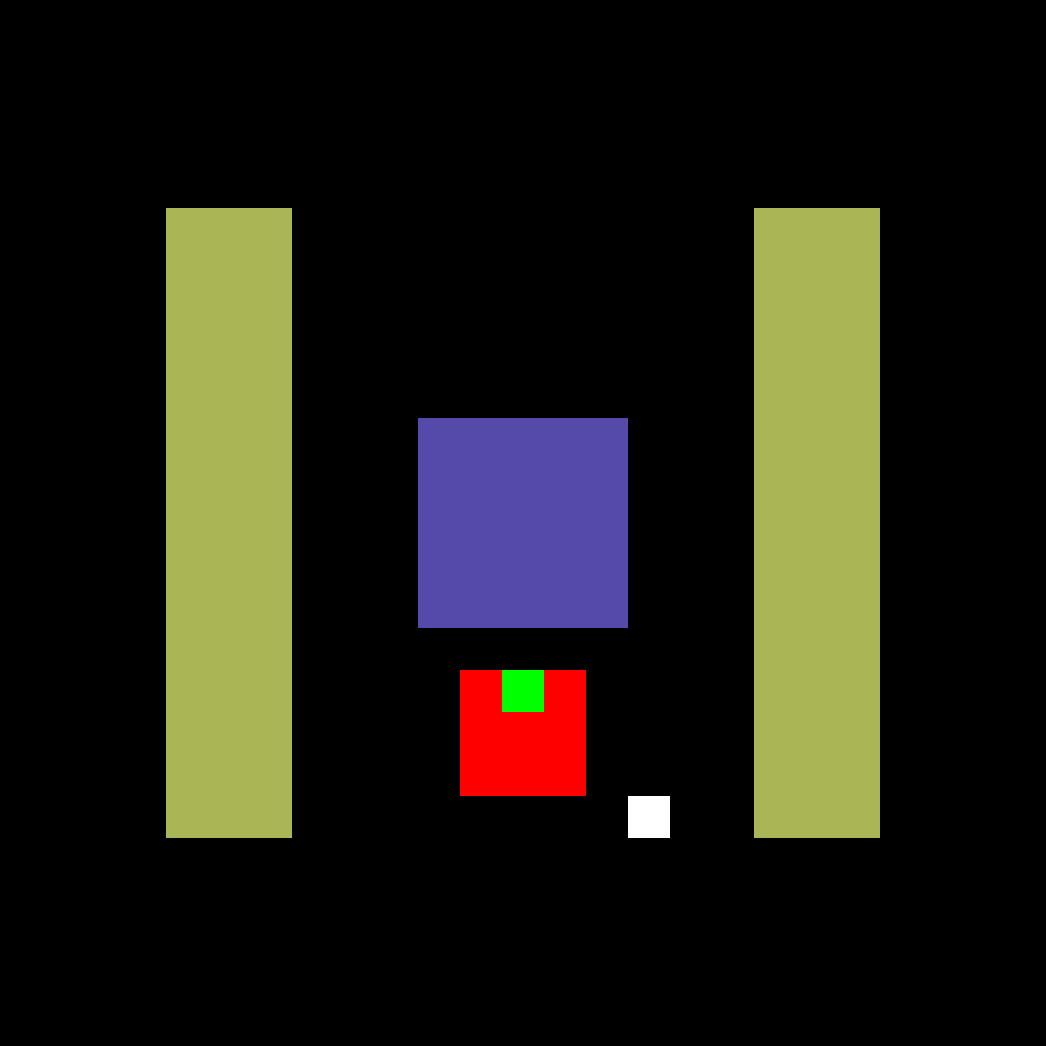
\includegraphics[width=55mm]{map_v.png}
      \caption{Rendu visuel de notre environnement \footnotemark}
    \end{minipage}
    \hfill%
    \begin{minipage}[c]{.37\linewidth}
      \centering
      \begin{itemize}
      \item Un environnement \textbf{discrétisé}
    \item Blanc pour le bateau
    \item Beige pour les murs
    \item Violet pour l'objectif
    \item Les cases rouges et vertes \textbf{montre les actions}
      \end{itemize}
    \end{minipage}
  \end{figure}
  \footnotetext{Les actions sont \textbf{seulement affichées pour l'utilisateur}, elle ne font pas parti de l'environnement}

\end{frame}

\begin{frame}

  \frametitle{Visuellement}

  \begin{figure}
    \begin{minipage}[c]{.46\linewidth}
      \centering
      

\tikzset{every picture/.style={line width=0.75pt}} %set default line width to 0.75pt        

\begin{tikzpicture}[x=0.75pt,y=0.75pt,yscale=-0.7,xscale=0.7]
%uncomment if require: \path (0,524); %set diagram left start at 0, and has height of 524

%Shape: Grid [id:dp47868985387811613] 
\draw  [draw opacity=0] (99.93,111) -- (380.5,111) -- (380.5,411.43) -- (99.93,411.43) -- cycle ; \draw  [color={rgb, 255:red, 0; green, 0; blue, 0 }  ,draw opacity=0.41 ] (99.93,111) -- (99.93,411.43)(119.93,111) -- (119.93,411.43)(139.93,111) -- (139.93,411.43)(159.93,111) -- (159.93,411.43)(179.93,111) -- (179.93,411.43)(199.93,111) -- (199.93,411.43)(219.93,111) -- (219.93,411.43)(239.93,111) -- (239.93,411.43)(259.93,111) -- (259.93,411.43)(279.93,111) -- (279.93,411.43)(299.93,111) -- (299.93,411.43)(319.93,111) -- (319.93,411.43)(339.93,111) -- (339.93,411.43)(359.93,111) -- (359.93,411.43)(379.93,111) -- (379.93,411.43) ; \draw  [color={rgb, 255:red, 0; green, 0; blue, 0 }  ,draw opacity=0.41 ] (99.93,111) -- (380.5,111)(99.93,131) -- (380.5,131)(99.93,151) -- (380.5,151)(99.93,171) -- (380.5,171)(99.93,191) -- (380.5,191)(99.93,211) -- (380.5,211)(99.93,231) -- (380.5,231)(99.93,251) -- (380.5,251)(99.93,271) -- (380.5,271)(99.93,291) -- (380.5,291)(99.93,311) -- (380.5,311)(99.93,331) -- (380.5,331)(99.93,351) -- (380.5,351)(99.93,371) -- (380.5,371)(99.93,391) -- (380.5,391)(99.93,411) -- (380.5,411) ; \draw  [color={rgb, 255:red, 0; green, 0; blue, 0 }  ,draw opacity=0.41 ]  ;
%Shape: Rectangle [id:dp028408793904989738] 
\draw  [color={rgb, 255:red, 0; green, 0; blue, 0 }  ,draw opacity=0 ][fill={rgb, 255:red, 255; green, 0; blue, 0 }  ,fill opacity=1 ] (160,371) -- (180,371) -- (180,391) -- (160,391) -- cycle ;
%Shape: Rectangle [id:dp3645945421789105] 
\draw  [color={rgb, 255:red, 0; green, 0; blue, 0 }  ,draw opacity=0 ][fill={rgb, 255:red, 255; green, 0; blue, 0 }  ,fill opacity=1 ] (140,351) -- (160,351) -- (160,371) -- (140,371) -- cycle ;
%Shape: Rectangle [id:dp36454377083997747] 
\draw  [color={rgb, 255:red, 0; green, 0; blue, 0 }  ,draw opacity=0 ][fill={rgb, 255:red, 255; green, 0; blue, 0 }  ,fill opacity=1 ] (140,311) -- (160,311) -- (160,331) -- (140,331) -- cycle ;
%Shape: Rectangle [id:dp15489044168337163] 
\draw  [color={rgb, 255:red, 0; green, 0; blue, 0 }  ,draw opacity=0 ][fill={rgb, 255:red, 255; green, 0; blue, 0 }  ,fill opacity=1 ] (160,251) -- (180,251) -- (180,271) -- (160,271) -- cycle ;
%Shape: Rectangle [id:dp8207759525539207] 
\draw  [color={rgb, 255:red, 0; green, 0; blue, 0 }  ,draw opacity=0 ][fill={rgb, 255:red, 255; green, 0; blue, 0 }  ,fill opacity=1 ] (200,211) -- (220,211) -- (220,231) -- (200,231) -- cycle ;
%Shape: Rectangle [id:dp8918625938006348] 
\draw  [color={rgb, 255:red, 0; green, 0; blue, 0 }  ,draw opacity=0 ][fill={rgb, 255:red, 255; green, 0; blue, 0 }  ,fill opacity=1 ] (260,171) -- (280,171) -- (280,191) -- (260,191) -- cycle ;
%Shape: Rectangle [id:dp18969414279703334] 
\draw  [color={rgb, 255:red, 0; green, 0; blue, 0 }  ,draw opacity=0 ][fill={rgb, 255:red, 255; green, 0; blue, 0 }  ,fill opacity=1 ] (340,131) -- (360,131) -- (360,151) -- (340,151) -- cycle ;
%Shape: Rectangle [id:dp6959162428957637] 
\draw  [color={rgb, 255:red, 0; green, 0; blue, 0 }  ,draw opacity=0 ][fill={rgb, 255:red, 80; green, 227; blue, 194 }  ,fill opacity=0.28 ] (140,351) -- (200,351) -- (200,411) -- (140,411) -- cycle ;
%Shape: Rectangle [id:dp8595893162029797] 
\draw  [color={rgb, 255:red, 0; green, 0; blue, 0 }  ,draw opacity=0 ][fill={rgb, 255:red, 80; green, 227; blue, 194 }  ,fill opacity=0.28 ] (100,311) -- (160,311) -- (160,371) -- (100,371) -- cycle ;
%Shape: Rectangle [id:dp7125139118142674] 
\draw  [color={rgb, 255:red, 0; green, 0; blue, 0 }  ,draw opacity=0 ][fill={rgb, 255:red, 80; green, 227; blue, 194 }  ,fill opacity=0.28 ] (120,251) -- (180,251) -- (180,311) -- (120,311) -- cycle ;
%Shape: Rectangle [id:dp5605542931365879] 
\draw  [color={rgb, 255:red, 0; green, 0; blue, 0 }  ,draw opacity=0 ][fill={rgb, 255:red, 80; green, 227; blue, 194 }  ,fill opacity=0.28 ] (160,171) -- (220,171) -- (220,231) -- (160,231) -- cycle ;
%Shape: Rectangle [id:dp13986117474891224] 
\draw  [color={rgb, 255:red, 0; green, 0; blue, 0 }  ,draw opacity=0 ][fill={rgb, 255:red, 80; green, 227; blue, 194 }  ,fill opacity=0.28 ] (220,151) -- (280,151) -- (280,211) -- (220,211) -- cycle ;
%Shape: Rectangle [id:dp414625732348471] 
\draw  [color={rgb, 255:red, 0; green, 0; blue, 0 }  ,draw opacity=0 ][fill={rgb, 255:red, 80; green, 227; blue, 194 }  ,fill opacity=0.28 ] (300,111) -- (360,111) -- (360,171) -- (300,171) -- cycle ;
%Shape: Rectangle [id:dp28561657100123994] 
\draw  [color={rgb, 255:red, 0; green, 0; blue, 0 }  ,draw opacity=0 ][fill={rgb, 255:red, 74; green, 144; blue, 226 }  ,fill opacity=0.43 ] (99.93,111) -- (220,111) -- (220,171) -- (99.93,171) -- cycle ;
%Shape: Rectangle [id:dp3467448199024483] 
\draw  [color={rgb, 255:red, 0; green, 0; blue, 0 }  ,draw opacity=0 ][fill={rgb, 255:red, 74; green, 144; blue, 226 }  ,fill opacity=0.43 ] (99.93,171) -- (160,171) -- (160,251) -- (99.93,251) -- cycle ;
%Shape: Rectangle [id:dp5695329224084911] 
\draw  [color={rgb, 255:red, 0; green, 0; blue, 0 }  ,draw opacity=0 ][fill={rgb, 255:red, 74; green, 144; blue, 226 }  ,fill opacity=0.43 ] (99.93,251) -- (119.93,251) -- (119.93,311) -- (99.93,311) -- cycle ;
%Shape: Rectangle [id:dp5130315302410975] 
\draw  [color={rgb, 255:red, 0; green, 0; blue, 0 }  ,draw opacity=0 ][fill={rgb, 255:red, 74; green, 144; blue, 226 }  ,fill opacity=0.43 ] (219.93,111) -- (299.93,111) -- (299.93,151) -- (219.93,151) -- cycle ;
%Shape: Rectangle [id:dp8108257305766648] 
\draw  [color={rgb, 255:red, 0; green, 0; blue, 0 }  ,draw opacity=0 ][fill={rgb, 255:red, 74; green, 144; blue, 226 }  ,fill opacity=0.43 ] (279.93,151) -- (300,151) -- (300,171) -- (279.93,171) -- cycle ;
%Shape: Rectangle [id:dp28577112744492084] 
\draw  [color={rgb, 255:red, 0; green, 0; blue, 0 }  ,draw opacity=0 ][fill={rgb, 255:red, 74; green, 144; blue, 226 }  ,fill opacity=0.43 ] (360,111) -- (379.93,111) -- (379.93,411) -- (360,411) -- cycle ;
%Shape: Rectangle [id:dp6220382285145605] 
\draw  [color={rgb, 255:red, 0; green, 0; blue, 0 }  ,draw opacity=0 ][fill={rgb, 255:red, 74; green, 144; blue, 226 }  ,fill opacity=0.43 ] (279.93,171) -- (360,171) -- (360,411) -- (279.93,411) -- cycle ;
%Shape: Rectangle [id:dp5579574046525082] 
\draw  [color={rgb, 255:red, 0; green, 0; blue, 0 }  ,draw opacity=0 ][fill={rgb, 255:red, 74; green, 144; blue, 226 }  ,fill opacity=0.43 ] (200,231) -- (280.07,231) -- (280.07,411) -- (200,411) -- cycle ;
%Shape: Rectangle [id:dp7482829542972489] 
\draw  [color={rgb, 255:red, 0; green, 0; blue, 0 }  ,draw opacity=0 ][fill={rgb, 255:red, 74; green, 144; blue, 226 }  ,fill opacity=0.43 ] (220,211) -- (280.07,211) -- (280.07,231) -- (220,231) -- cycle ;
%Shape: Rectangle [id:dp7193082143482312] 
\draw  [color={rgb, 255:red, 0; green, 0; blue, 0 }  ,draw opacity=0 ][fill={rgb, 255:red, 74; green, 144; blue, 226 }  ,fill opacity=0.43 ] (179.93,231) -- (199.93,231) -- (199.93,311) -- (179.93,311) -- cycle ;
%Shape: Rectangle [id:dp6413839794315745] 
\draw  [color={rgb, 255:red, 0; green, 0; blue, 0 }  ,draw opacity=0 ][fill={rgb, 255:red, 74; green, 144; blue, 226 }  ,fill opacity=0.43 ] (159.93,231) -- (179.93,231) -- (179.93,251) -- (159.93,251) -- cycle ;
%Shape: Rectangle [id:dp6543722862974133] 
\draw  [color={rgb, 255:red, 0; green, 0; blue, 0 }  ,draw opacity=0 ][fill={rgb, 255:red, 74; green, 144; blue, 226 }  ,fill opacity=0.43 ] (159.93,311) -- (200,311) -- (200,351) -- (159.93,351) -- cycle ;
%Shape: Rectangle [id:dp5968474102033507] 
\draw  [color={rgb, 255:red, 0; green, 0; blue, 0 }  ,draw opacity=0 ][fill={rgb, 255:red, 74; green, 144; blue, 226 }  ,fill opacity=0.43 ] (100,371) -- (140.07,371) -- (140.07,411) -- (100,411) -- cycle ;
%Straight Lines [id:da9777313804077001] 
\draw [color={rgb, 255:red, 189; green, 16; blue, 224 }  ,draw opacity=0.81 ]   (334.1,131.2) -- (320.1,144.2) ;
%Straight Lines [id:da08076985066570086] 
\draw [color={rgb, 255:red, 189; green, 16; blue, 224 }  ,draw opacity=0.81 ]   (340.1,134.2) -- (323.1,151.2) ;
%Straight Lines [id:da10279614851476837] 
\draw [color={rgb, 255:red, 189; green, 16; blue, 224 }  ,draw opacity=0.81 ]   (340.1,143.2) -- (332.1,151.2) ;
%Straight Lines [id:da8251437903055174] 
\draw [color={rgb, 255:red, 189; green, 16; blue, 224 }  ,draw opacity=0.81 ]   (338.1,151.2) ;
%Straight Lines [id:da357129254928066] 
\draw [color={rgb, 255:red, 189; green, 16; blue, 224 }  ,draw opacity=0.81 ]   (325.1,131.2) -- (320.1,136.2) ;
%Straight Lines [id:da4131562105376825] 
\draw [color={rgb, 255:red, 189; green, 16; blue, 224 }  ,draw opacity=0.81 ]   (254.1,171.2) -- (240.1,184.2) ;
%Straight Lines [id:da8507776871178556] 
\draw [color={rgb, 255:red, 189; green, 16; blue, 224 }  ,draw opacity=0.81 ]   (260.1,174.2) -- (243.1,191.2) ;
%Straight Lines [id:da006092988666045018] 
\draw [color={rgb, 255:red, 189; green, 16; blue, 224 }  ,draw opacity=0.81 ]   (260.1,183.2) -- (252.1,191.2) ;
%Straight Lines [id:da7825038507901239] 
\draw [color={rgb, 255:red, 189; green, 16; blue, 224 }  ,draw opacity=0.81 ]   (258.1,191.2) ;
%Straight Lines [id:da3304543035440064] 
\draw [color={rgb, 255:red, 189; green, 16; blue, 224 }  ,draw opacity=0.81 ]   (245.1,171.2) -- (240.1,176.2) ;
%Straight Lines [id:da06122494845742721] 
\draw [color={rgb, 255:red, 189; green, 16; blue, 224 }  ,draw opacity=0.81 ]   (194.1,191.2) -- (180.1,204.2) ;
%Straight Lines [id:da329018065517686] 
\draw [color={rgb, 255:red, 189; green, 16; blue, 224 }  ,draw opacity=0.81 ]   (200.1,194.2) -- (183.1,211.2) ;
%Straight Lines [id:da1868218724945636] 
\draw [color={rgb, 255:red, 189; green, 16; blue, 224 }  ,draw opacity=0.81 ]   (200.1,203.2) -- (192.1,211.2) ;
%Straight Lines [id:da47428667662448865] 
\draw [color={rgb, 255:red, 189; green, 16; blue, 224 }  ,draw opacity=0.81 ]   (198.1,211.2) ;
%Straight Lines [id:da7888749387544363] 
\draw [color={rgb, 255:red, 189; green, 16; blue, 224 }  ,draw opacity=0.81 ]   (185.1,191.2) -- (180.1,196.2) ;
%Straight Lines [id:da5426460500043468] 
\draw [color={rgb, 255:red, 189; green, 16; blue, 224 }  ,draw opacity=0.81 ]   (154.1,271.2) -- (140.1,284.2) ;
%Straight Lines [id:da9612689358112596] 
\draw [color={rgb, 255:red, 189; green, 16; blue, 224 }  ,draw opacity=0.81 ]   (160.1,274.2) -- (143.1,291.2) ;
%Straight Lines [id:da763255566176499] 
\draw [color={rgb, 255:red, 189; green, 16; blue, 224 }  ,draw opacity=0.81 ]   (160.1,283.2) -- (152.1,291.2) ;
%Straight Lines [id:da8252731441535606] 
\draw [color={rgb, 255:red, 189; green, 16; blue, 224 }  ,draw opacity=0.81 ]   (158.1,291.2) ;
%Straight Lines [id:da3161738220685639] 
\draw [color={rgb, 255:red, 189; green, 16; blue, 224 }  ,draw opacity=0.81 ]   (145.1,271.2) -- (140.1,276.2) ;
%Straight Lines [id:da5130752531860867] 
\draw [color={rgb, 255:red, 189; green, 16; blue, 224 }  ,draw opacity=0.81 ]   (134.1,331.2) -- (120.1,344.2) ;
%Straight Lines [id:da06175262743667553] 
\draw [color={rgb, 255:red, 189; green, 16; blue, 224 }  ,draw opacity=0.81 ]   (140.1,334.2) -- (123.1,351.2) ;
%Straight Lines [id:da8682630447762676] 
\draw [color={rgb, 255:red, 189; green, 16; blue, 224 }  ,draw opacity=0.81 ]   (140.1,343.2) -- (132.1,351.2) ;
%Straight Lines [id:da8157074457761089] 
\draw [color={rgb, 255:red, 189; green, 16; blue, 224 }  ,draw opacity=0.81 ]   (138.1,351.2) ;
%Straight Lines [id:da946308372929793] 
\draw [color={rgb, 255:red, 189; green, 16; blue, 224 }  ,draw opacity=0.81 ]   (125.1,331.2) -- (120.1,336.2) ;
%Straight Lines [id:da7525726280467624] 
\draw [color={rgb, 255:red, 189; green, 16; blue, 224 }  ,draw opacity=0.81 ]   (174.1,371.2) -- (160.1,384.2) ;
%Straight Lines [id:da8692101321164531] 
\draw [color={rgb, 255:red, 189; green, 16; blue, 224 }  ,draw opacity=0.81 ]   (180.1,374.2) -- (163.1,391.2) ;
%Straight Lines [id:da17255630437420355] 
\draw [color={rgb, 255:red, 189; green, 16; blue, 224 }  ,draw opacity=0.81 ]   (180.1,383.2) -- (172.1,391.2) ;
%Straight Lines [id:da41595632994048626] 
\draw [color={rgb, 255:red, 189; green, 16; blue, 224 }  ,draw opacity=0.81 ]   (178.1,391.2) ;
%Straight Lines [id:da16638093291732559] 
\draw [color={rgb, 255:red, 189; green, 16; blue, 224 }  ,draw opacity=0.81 ]   (165.1,371.2) -- (160.1,376.2) ;

% Text Node
\draw (170,381) node   [align=left] {t0};
% Text Node
\draw (150,361) node   [align=left] {t1};
% Text Node
\draw (150,321) node   [align=left] {t2};
% Text Node
\draw (170,261) node   [align=left] {t3};
% Text Node
\draw (210,221) node   [align=left] {t3};
% Text Node
\draw (270,181) node   [align=left] {t4};
% Text Node
\draw (350,141) node   [align=left] {t5};


\end{tikzpicture}

      \caption{Exemple de trajectoire de bateau}
    \end{minipage}
    \hfill%
    \begin{minipage}[c]{.46\linewidth}
      \centering
      \begin{itemize}
      \item En {\color{red} rouge} les positions successives du bateau
      \item En {\color{purple} violet}, prise en compte de l'inertie (répétition du déplacement)
      \item En {\color{green} vert} les choix d'actions successifs (rayon 1 de autour de {\color{purple}violet} \footnotemark)
      \item Sous python, \textbf{Numpy} permet la \textbf{vectorisation} et donc les \textbf{parties simultanées} (1000 parties prennent le même temps que une ou deux parties)
      \end{itemize}
    \end{minipage}
  \end{figure}
  \footnotetext{Ici, la zone est carré mais la forme peut varier pour augmenter l'aspect réaliste du modèle et s'adapter au caractéristique même du bateau.}

\end{frame}


\section{Le Policy Gradients}

\subsection{La théorie}

\begin{frame}

  \frametitle{Définissions et notations}

  \begin{block}{La Politique et ses fonctions Gain, Q-Value, Value et Reward associées}
    \begin{itemize}
    \item La Politique
      \begin{equation} \pi_{\theta}(s) = (p_i)_{i \in \llbracket 1, ac \rrbracket} / {\scalebox{0.85}{$\displaystyle \sum_{i = 1}^{ac}$}}p_i = 1  \end{equation}
    \item Le Gain
      \begin{equation} G_t = {\scalebox{0.85}{$\displaystyle \sum_{k=0}^{\infty}$}} \gamma^k R_{t+k+1} \end{equation}
    \item La Q-value
      \begin{equation} Q^\pi(s, a) = \mathbb{E}_{a\sim \pi} [G_t \vert S_t = s, A_t = a] \end{equation}
    \item La Value
      \begin{equation} V^\pi (s) = \mathbb{E}_{a\sim \pi} [G_t \vert S_t = s] \end{equation}
    \item La Recompense, fonction Reward
      \begin{equation} J(\theta) 
= {\scalebox{0.85}{$\displaystyle \sum_{s \in \mathcal{S}}$}} d^\pi(s) V^\pi(s) 
= {\scalebox{0.85}{$\displaystyle \sum_{s \in \mathcal{S}}$}} d^\pi(s) {\scalebox{0.85}{$\displaystyle  \sum_{a \in \mathcal{A}}$}} \pi_\theta(a \vert s) Q^\pi(s, a) \end{equation}
    \end{itemize}
  \end{block}
  
\end{frame}

\begin{frame}[label=retourCNN]

  \frametitle{La Politique}

  \begin{block}{Un réseaux de neuronnes de convolution maison\footnotemark pour $\pi_{\theta}(s)$}
    \begin{itemize}
    \item $s$ correspond à l'entrée
    \item $\pi_{\theta}(s)$ correspond à la sortie
    \item $\theta$ correspond aux poids et biais du réseaux
    \end{itemize}

  \end{block}

  \begin{figure}
    
    \begin{minipage}[c]{.28\linewidth}
      \centering
      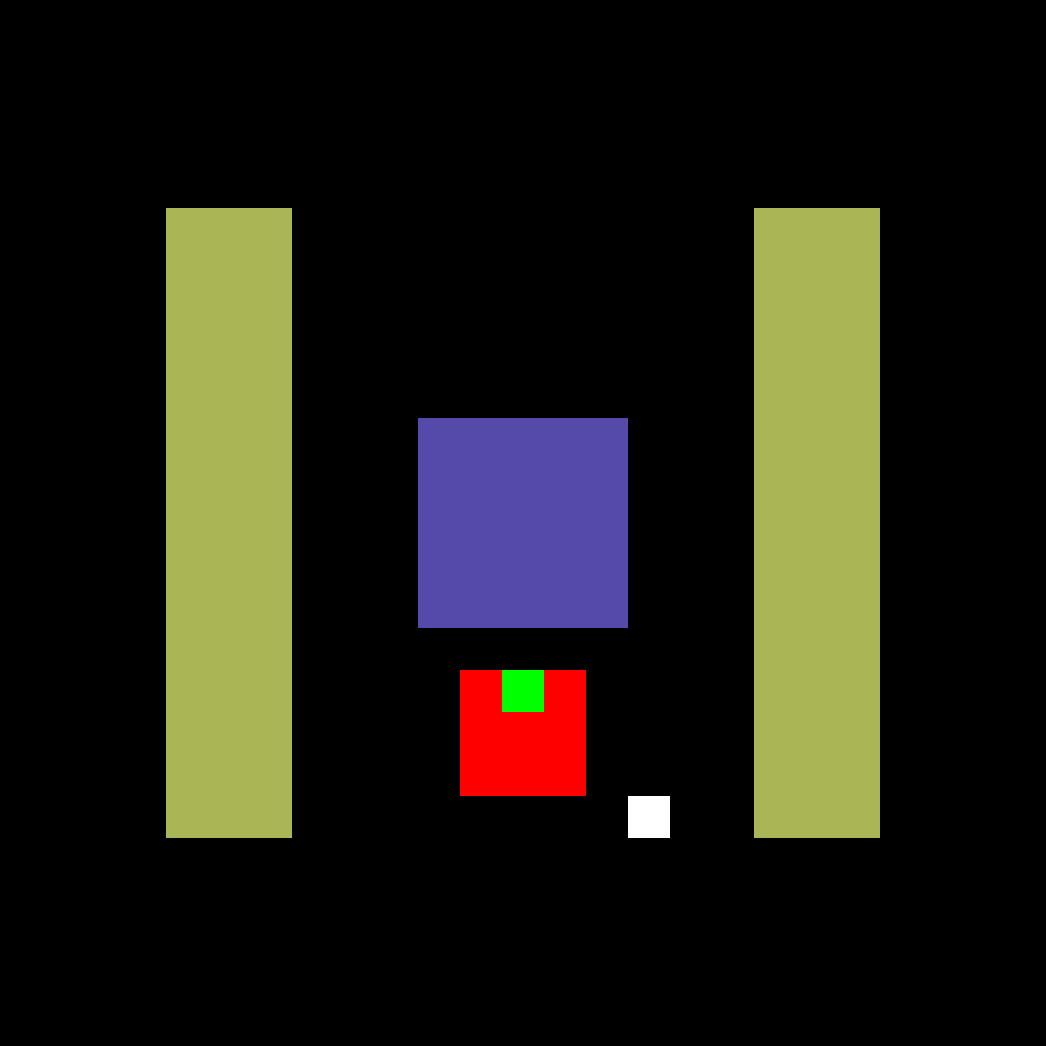
\includegraphics[width=\linewidth]{map_v.png}
    \end{minipage}
    \hfill%
    \begin{minipage}[c]{.04\linewidth}
      \centering
      $=$
    \end{minipage}
    \hfill%
    \begin{minipage}[c]{.43\linewidth}
      \centering
      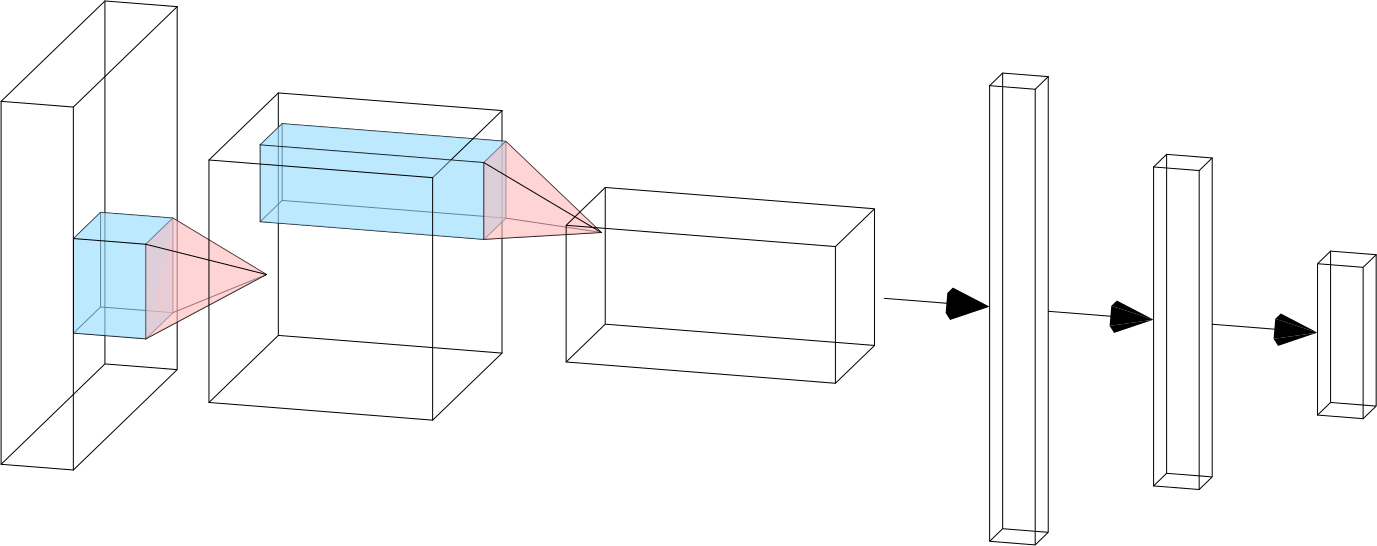
\includegraphics[width=1.05\linewidth]{CNN.png}
    \end{minipage}
    \hfill%
    \begin{minipage}[c]{.218\linewidth}
      \centering \[ =
      \left[
      \begin{array}{c}
        {\color{red}0.01}\\
        {\color{green} 0.85}\\
        {\color{red}0.01}\\
        {\color{red}0.03}\\
        {\color{red}0.04}\\
        {\color{red}0.01}\\
        {\color{red}0.02}\\
        {\color{red}0.01}\\
        {\color{red}0.02}
      \end{array}
      \right] \]
    \end{minipage}
  \end{figure}
  \footnotetext{Nous utilisons ici \hyperlink{CNN}{notre implémentation sans librairies spécialisées du Convolutional Neural Network}}
\end{frame}

\begin{frame}[label=policyintroduction]
  \frametitle{L'entrainement}
  \begin{block}{L'initialisation}
    On définit une structure pour le réseau de neurones où les poids et biais sont définis aléatoirement
  \end{block}

  \begin{block}{Par récurrence (En époques) \footnotemark}
    \begin{itemize}
    \item On effectue P parties en parallèle, on récupère:
      \begin{center}
      {\scalebox{0.85}{
      $\left\{
      \begin{array}{c}
        S_0^1, A_0^1, R_0^1, \cdots, S_{f_1-1}^1, A_{f_1-1}^1, R_{f_1-1}^1, S^1_{f_1} \\
        \vdots \\
        S_0^P, A_0^P, R_0^P, \cdots, S_{f_P-1}^P, A_{f_P-1}^P, R_{f_P-1}^P, S^P_{f_P} 
      \end{array}
      \right. $}} \end{center}
    \item Pour tout $i \in \llbracket 1, P \rrbracket$ et $t \in \llbracket 0, f_i - 1 \rrbracket$
      \begin{align}
        G_t^i &= {\scalebox{0.85}{$\displaystyle \sum_{k=O}^{f_i-t-2}$}} \gamma^k R^i_{t+k+1} \\
        \theta &\leftarrow \theta + \alpha \gamma^t G^i_t \nabla_\theta \ln \pi_\theta(A^i_t \vert S^i_t)
      \end{align}
    
    \end{itemize}

  \end{block}

  \footnotetext{Ceci résulte d'un \hyperlink{demopolicygradient}{théorème majeur sur le Policy Gradients}}
\end{frame}

\subsection{Résultats}

\begin{frame}

\end{frame}

\section*{Conclusion}

\subsection{Objectif}

\subsection{Ouverture}

\appendix

\section*{Notre implémentation du CNN}

\begin{frame}[label=CNN]
  \frametitle{Un fait maison}
  \hyperlink{retourCNN}{Retour}
\end{frame}

\section*{Proof of the Policy Gradient Theroem}

\begin{frame}[label=demopolicygradient]
  \frametitle{Bonsoir ici on se marre}

  \hyperlink{policyintroduction}{Retour}
  
  klbuerbqhvhjbyerukbvhjqkjbrey
\end{frame}
\end{document}

